
\chapter{Results and Discussion}
\begin{refsection}

The data gathered during the study are presented and evaluated in this chapter. A discussion and thorough analysis of helmet compliance, wrong helmet use, and motorcycle overloading are also included in this chapter.
\begin{refsection}

\section{Data Collection}
\subsection{Data Gathering}
The researchers searched for datasets that included motorcycles, not motorcycles, persons with no helmet, persons with proper helmets, and persons with wrong helmet use. While it was easy to find images for motorcycles, not motorcycles, no-helmet, and proper-helmet categories, finding enough images for wrong helmet use was challenging. To create the dataset, the researchers used a phone to capture images of riders and used some images from the internet. In total, the dataset consists of around 1,133 images covering all categories. Before training the model, the images were preprocessed. This included resizing all images to a standard input size, labeling each image with bounding boxes for motorcycles and riders, and applying data augmentation techniques such as flipping, blurring, rotation, brightness adjustment, adding noise, and cropping to increase variability. The pixel values of the images were normalized to improve model training, and the dataset was split into training, validation, and test sets to allow proper evaluation of the model’s performance.

\begin{figure}[H]
\centering
\begin{tabular}{|c|c|c|}
\hline
Motorcycle & Not motorcycle & Person with no helmet \\
\hline
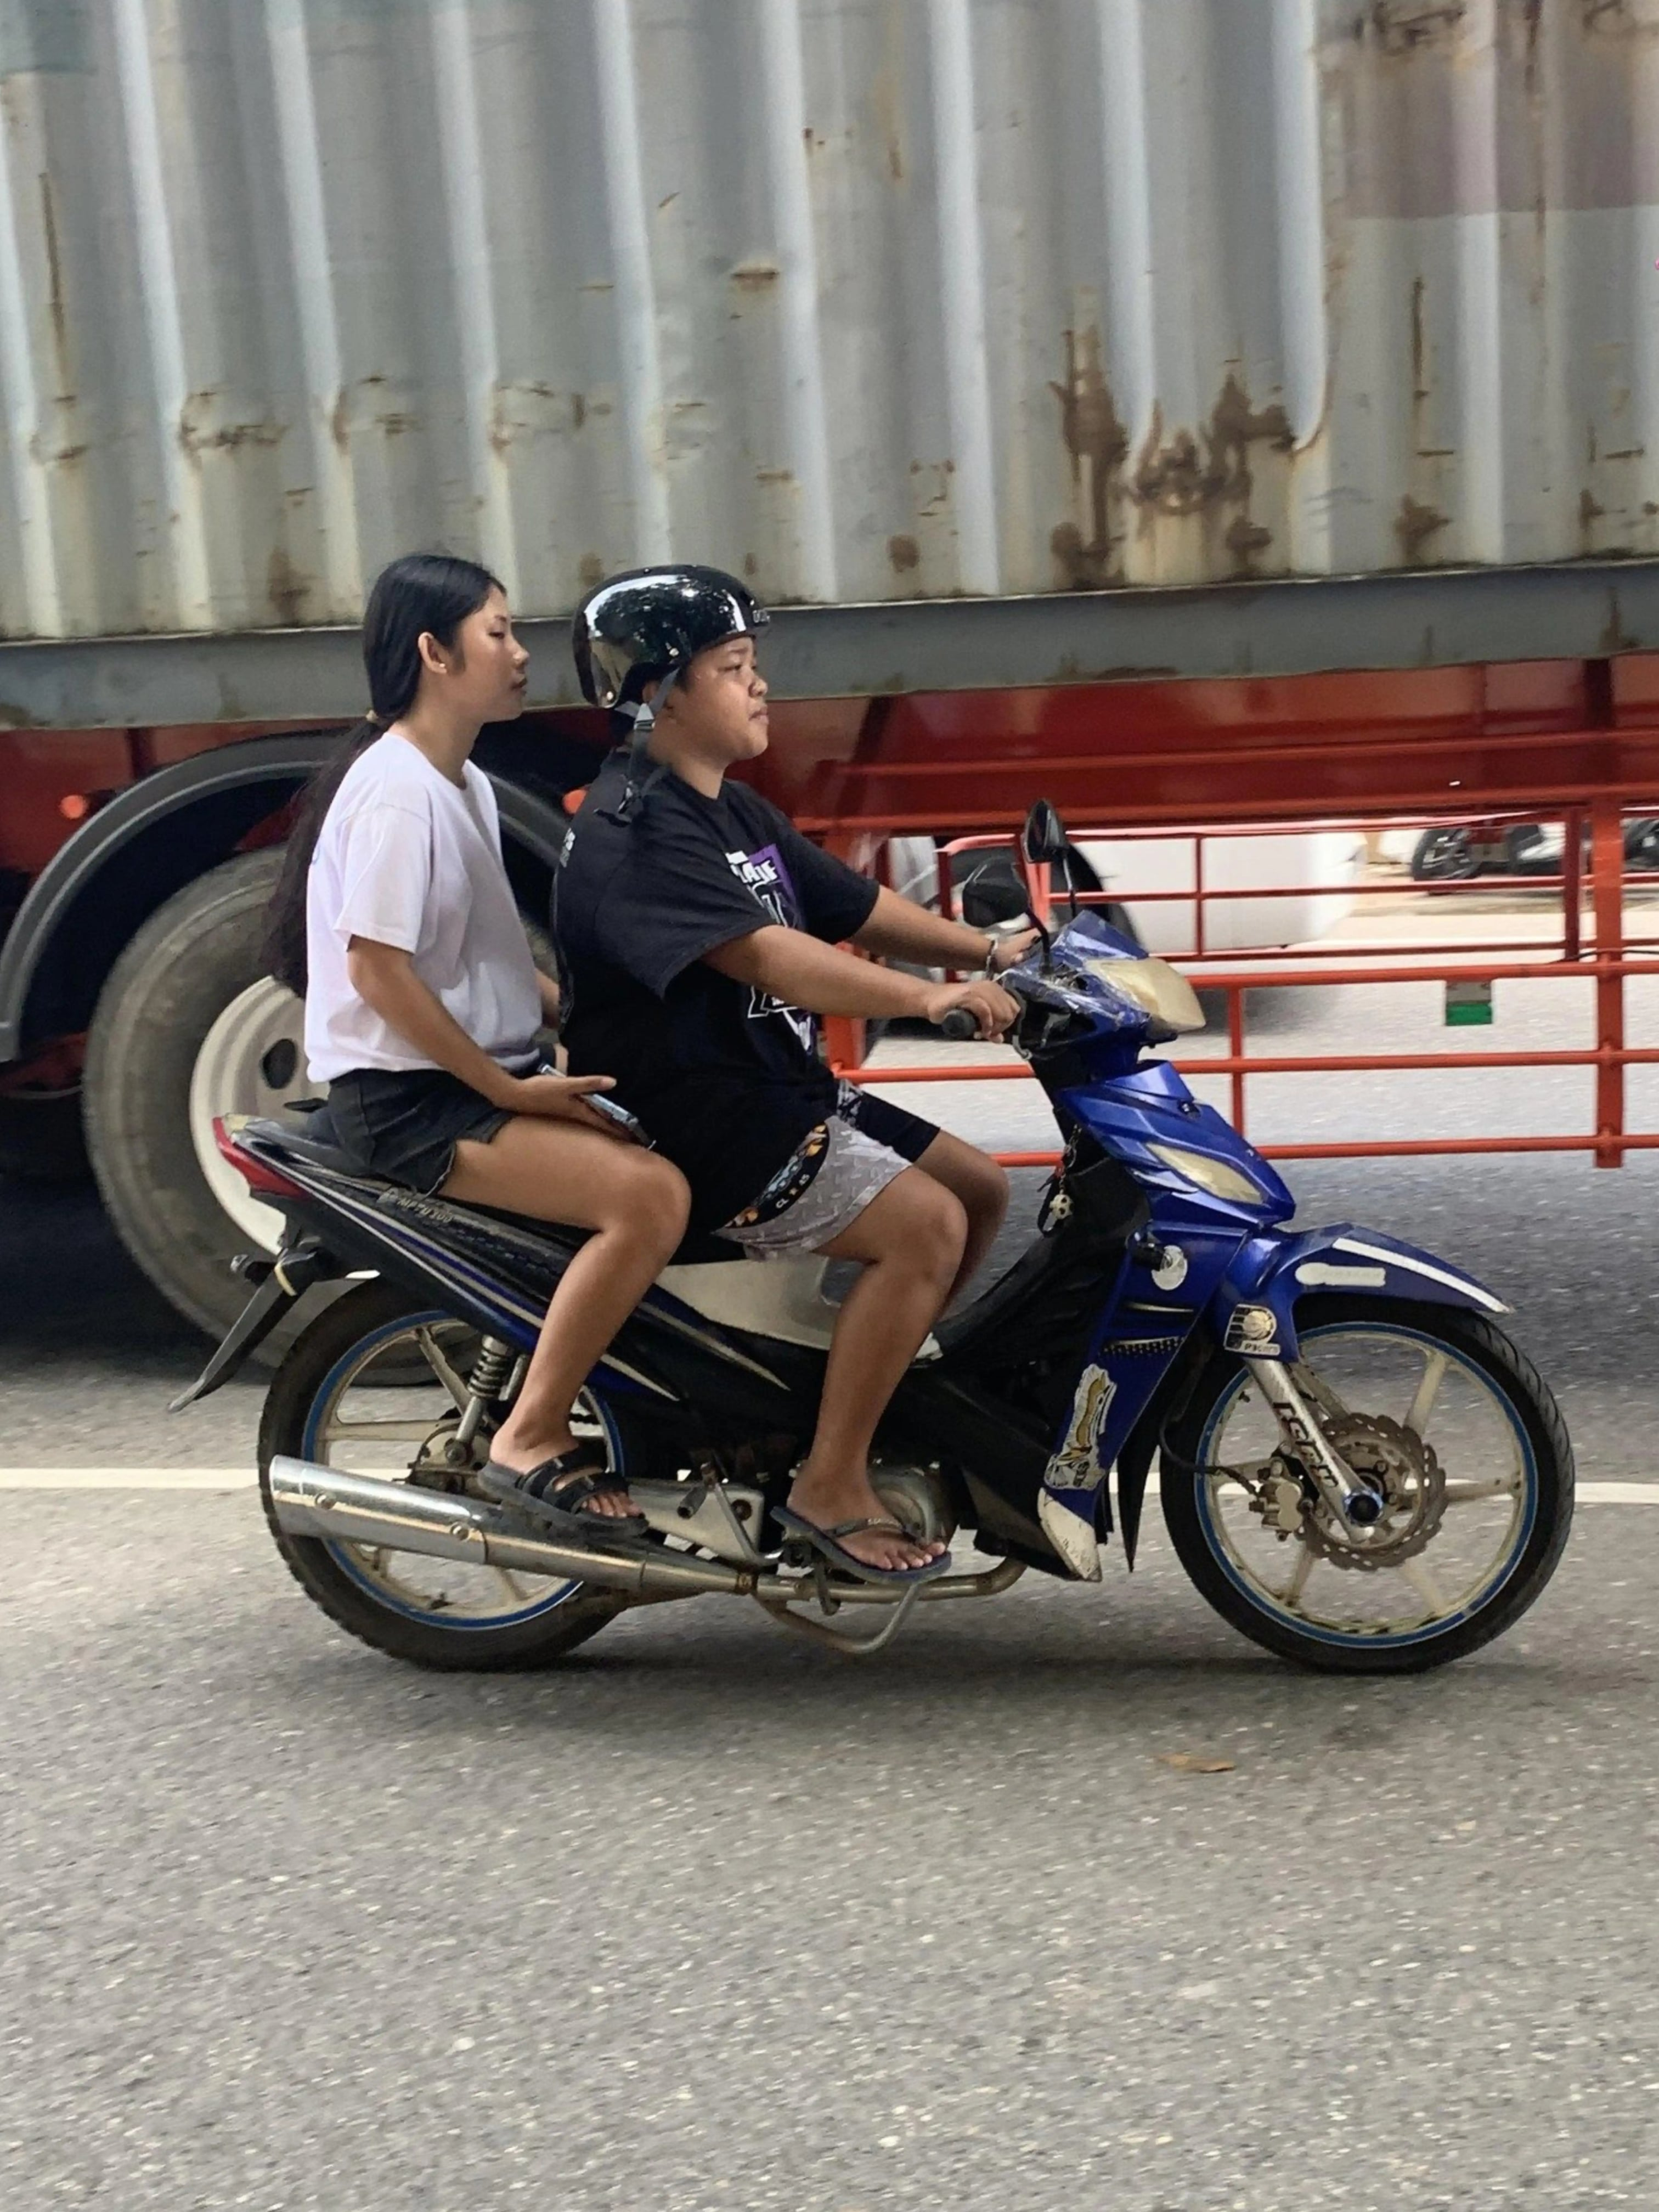
\includegraphics[width=0.28\textwidth]{figures/Fig 7.png} & 
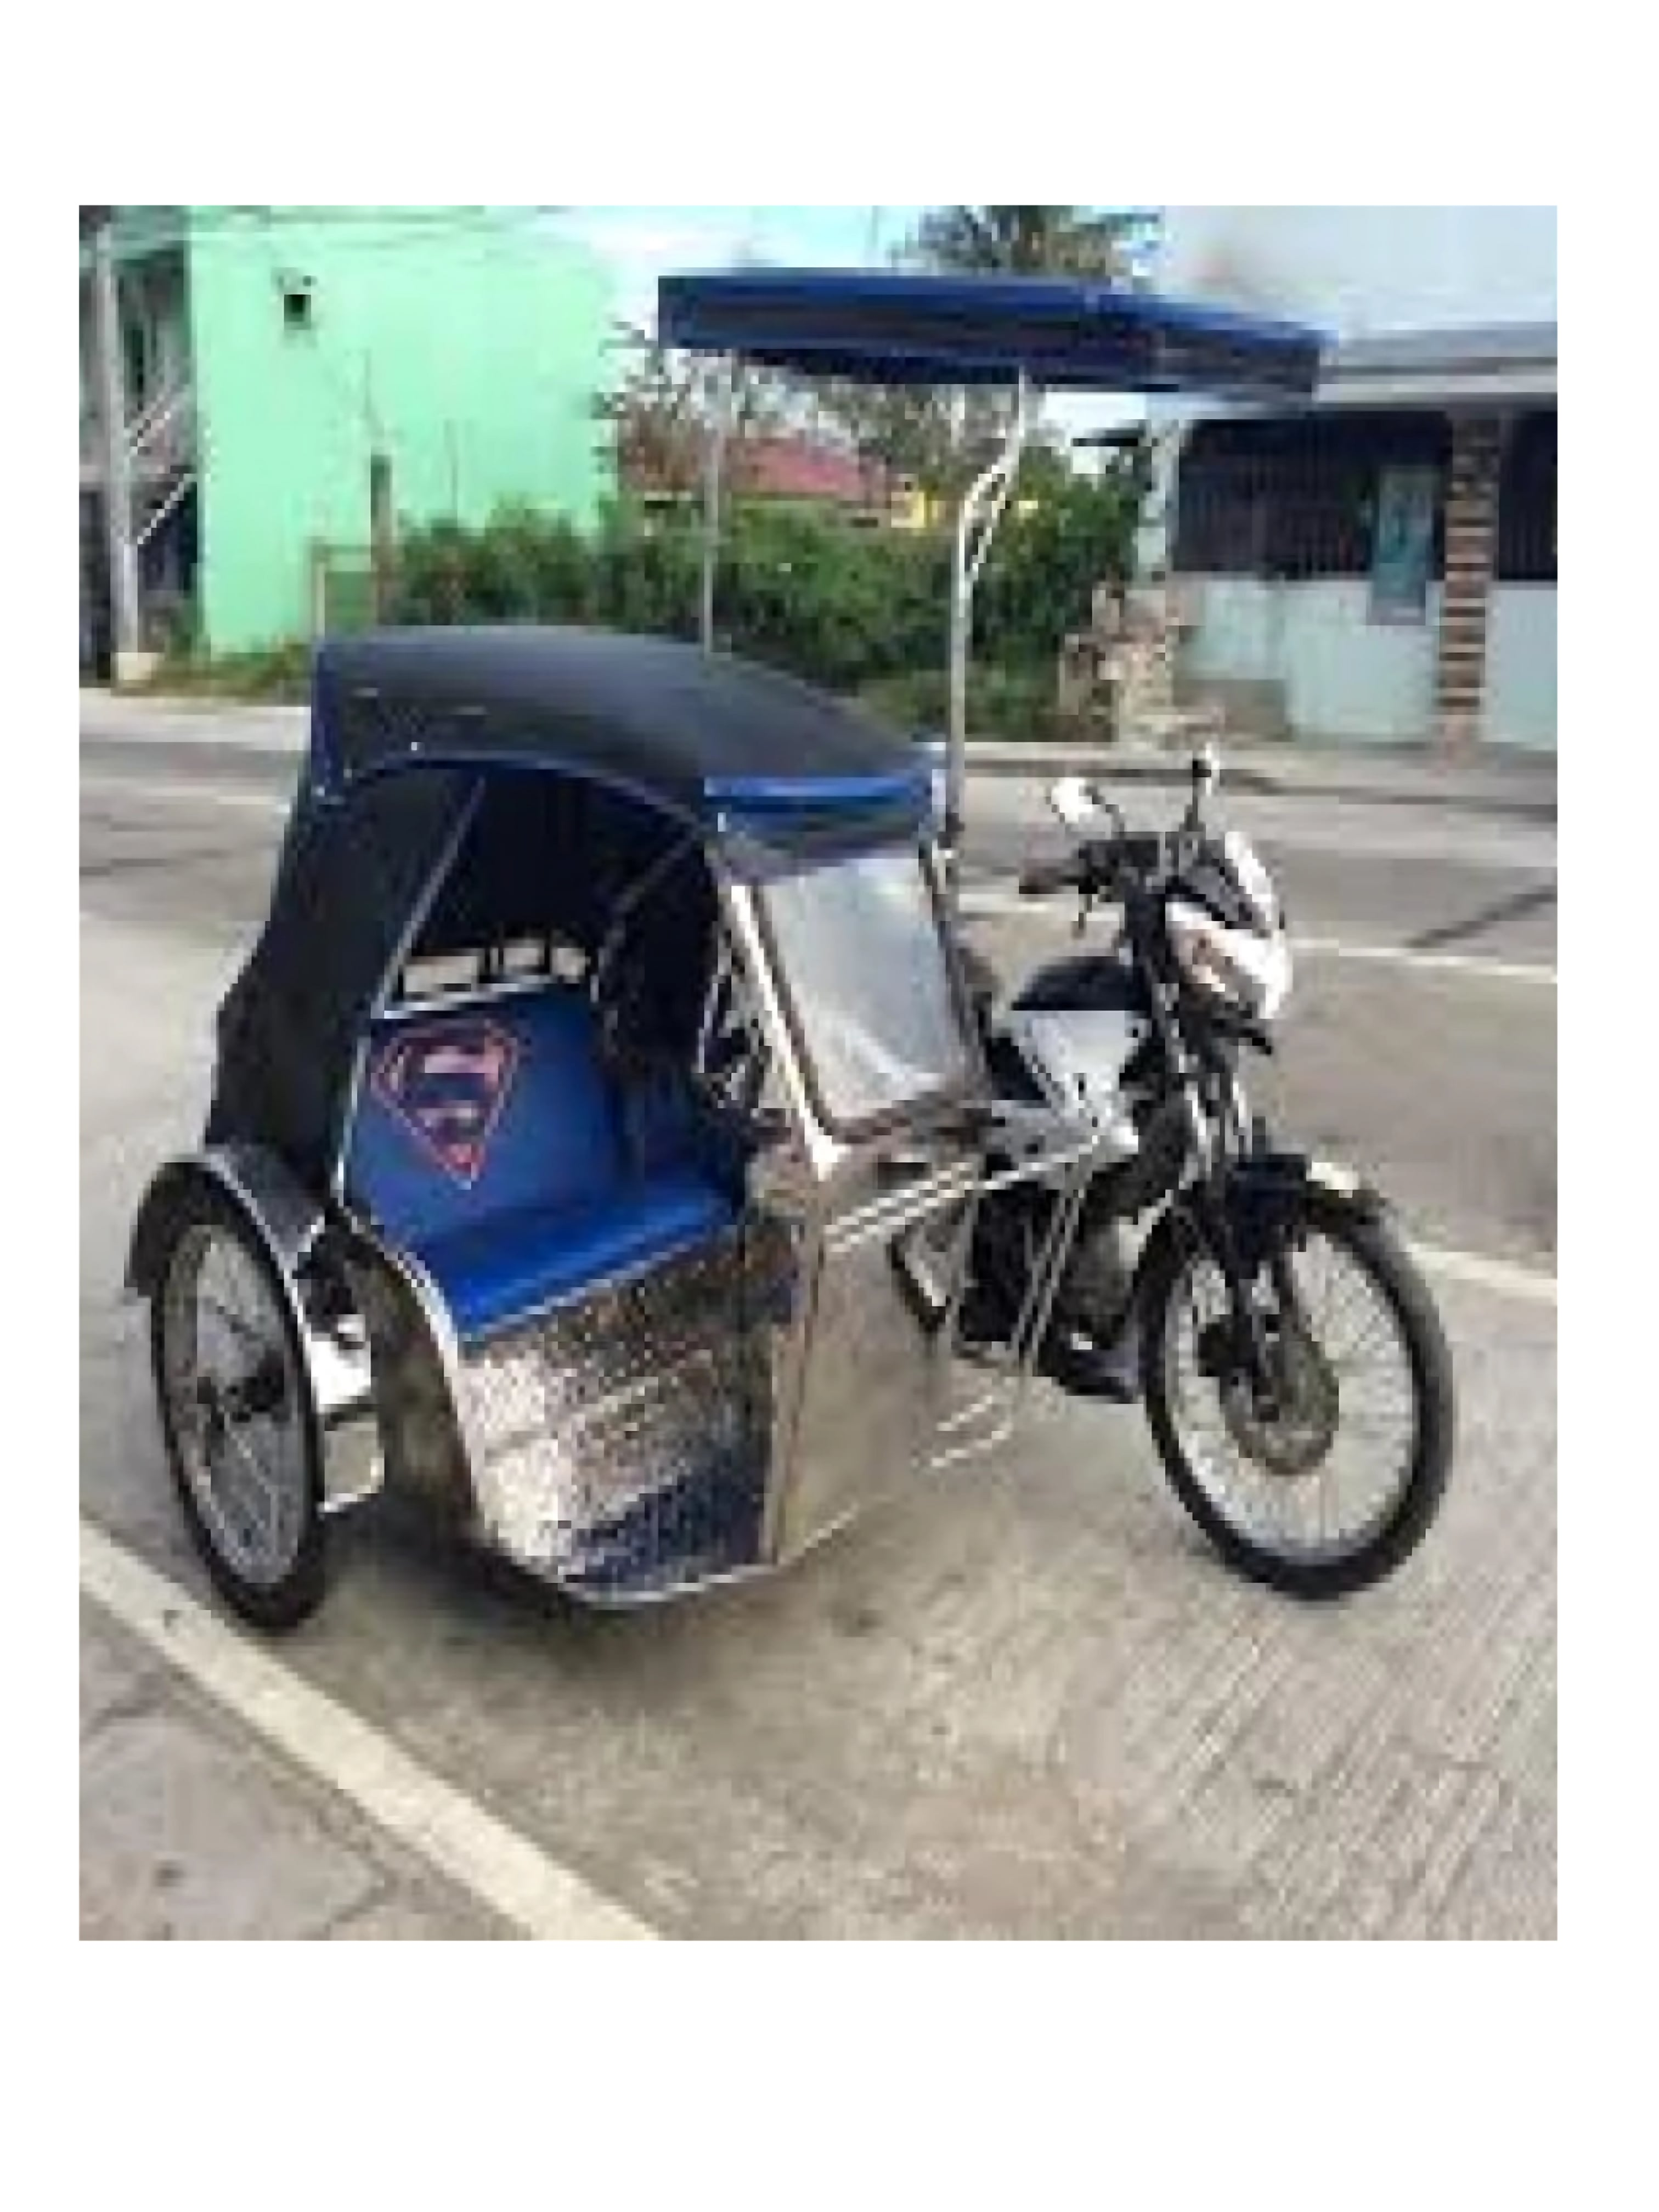
\includegraphics[width=0.28\textwidth]{figures/Fig 8.png} & 
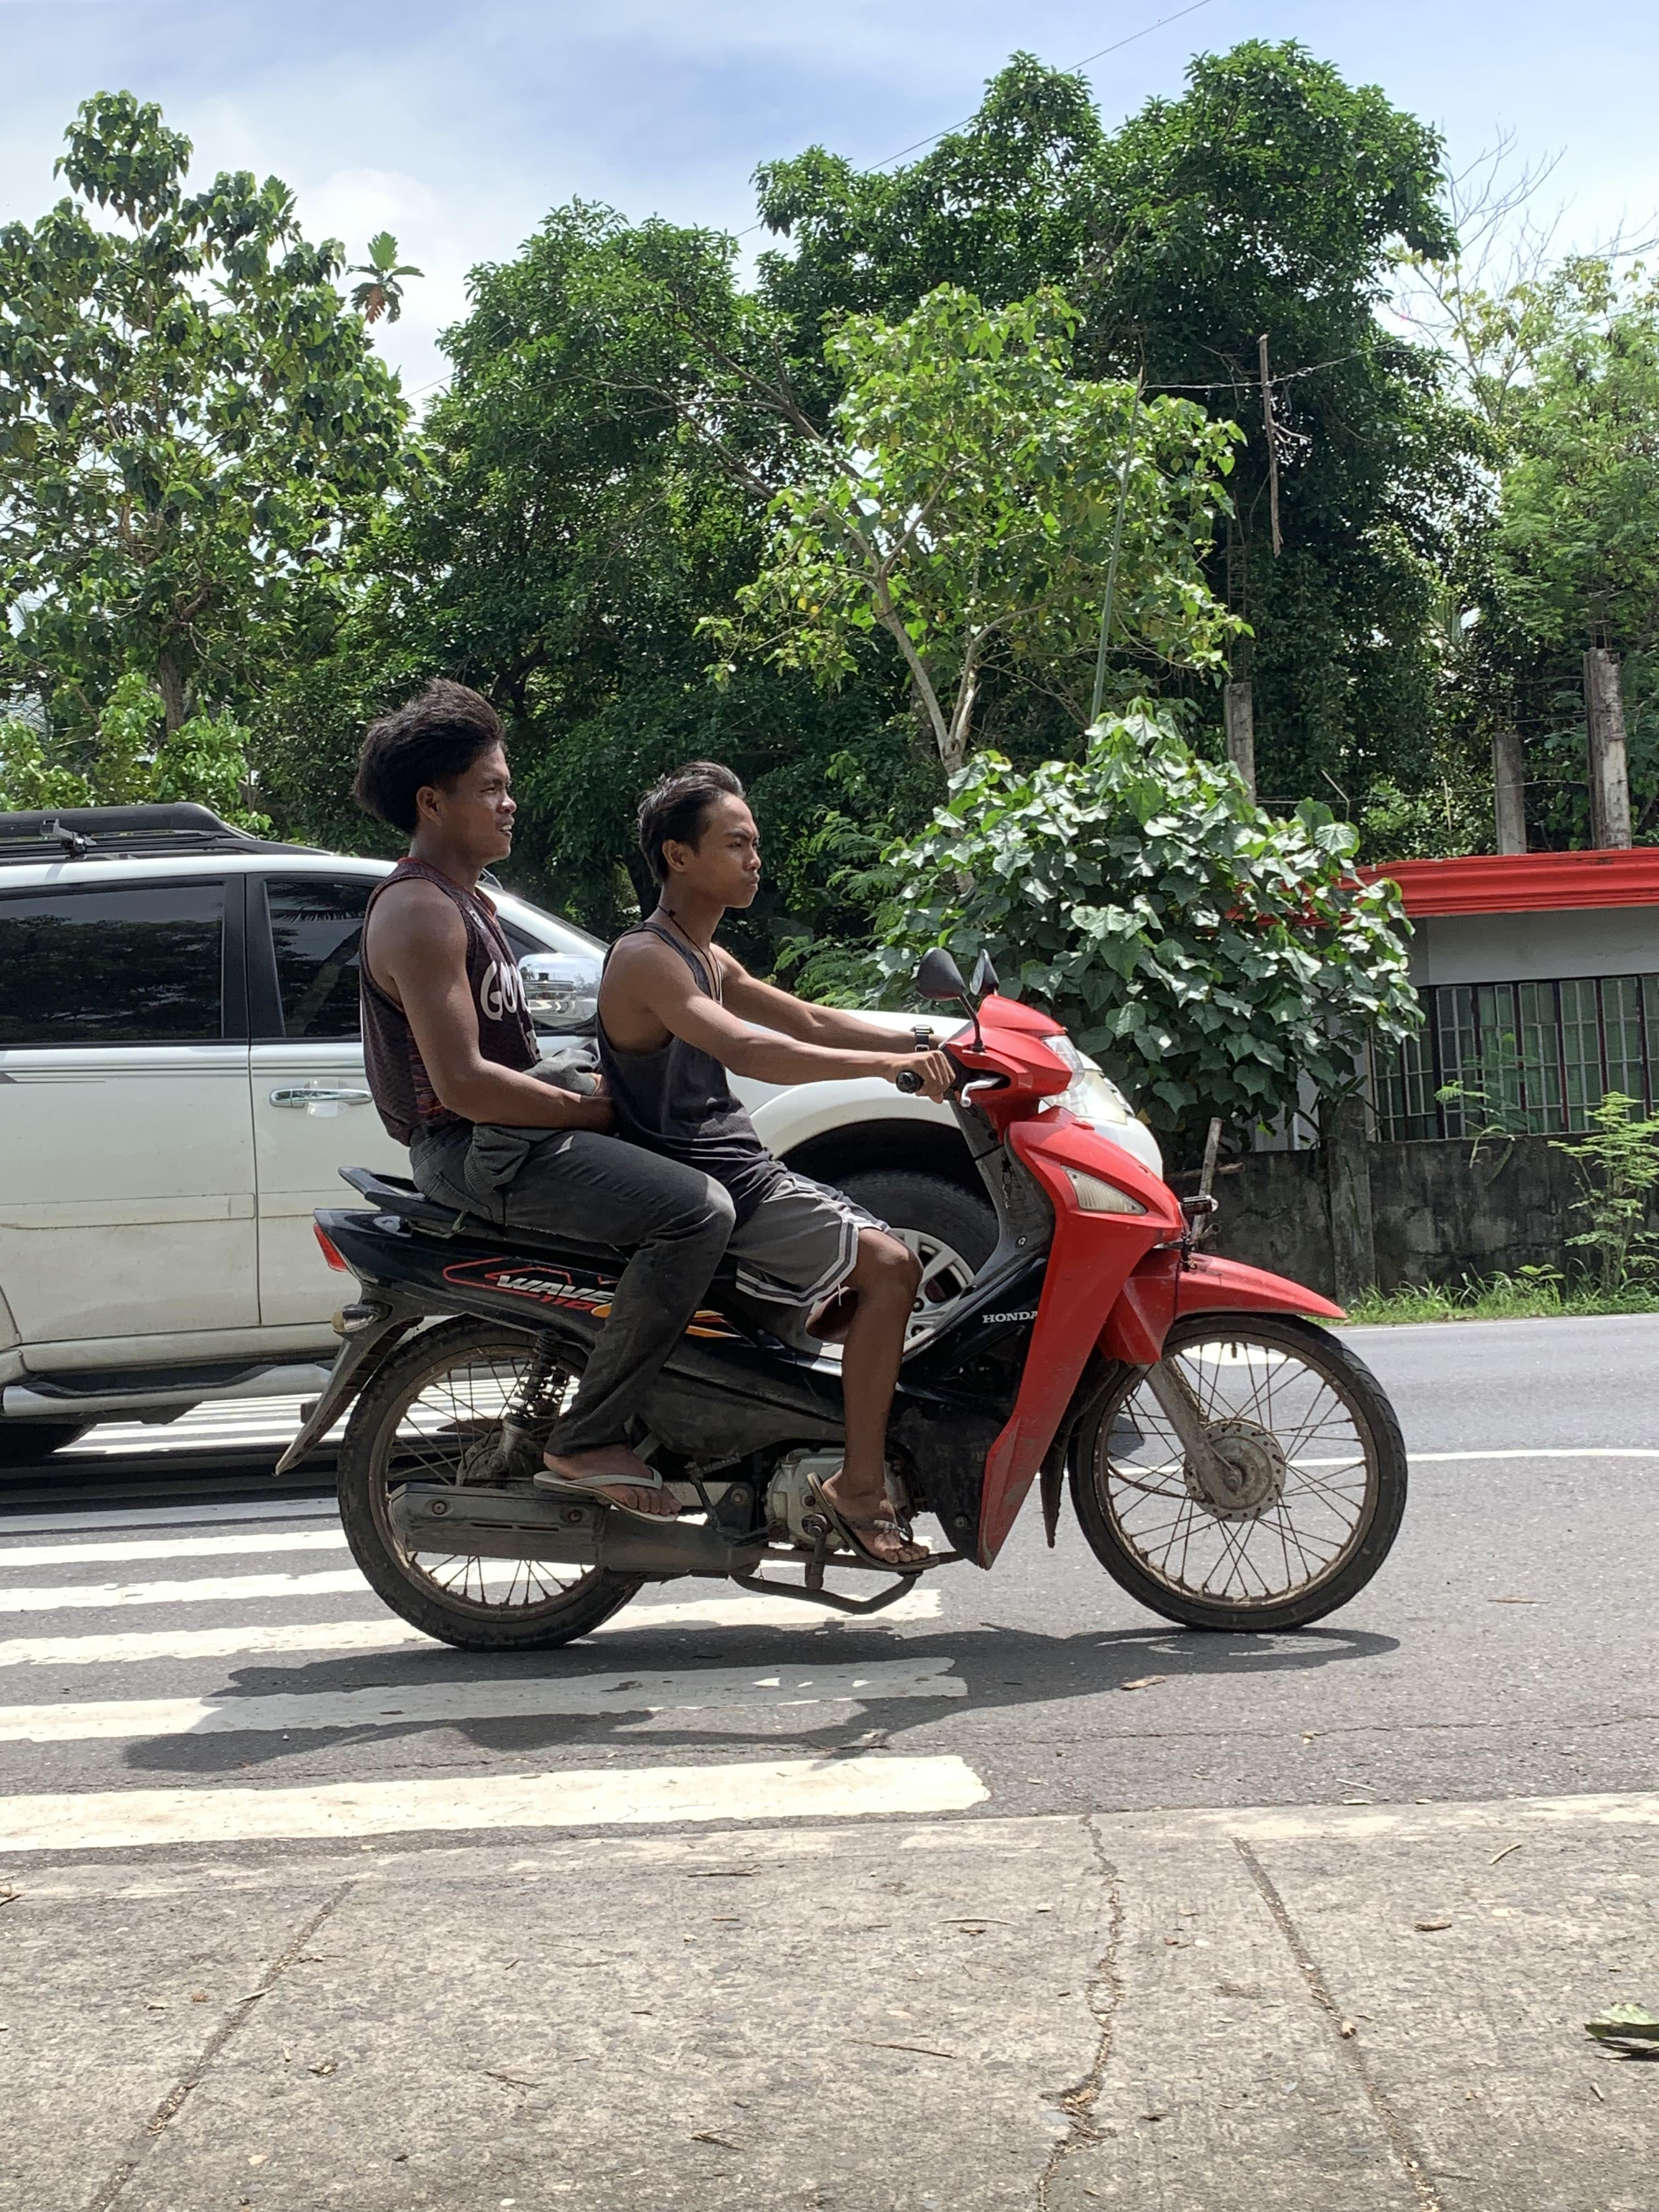
\includegraphics[width=0.28\textwidth]{figures/Fig 9.png} \\
\hline
\end{tabular}

\vspace{0.3cm} % space between rows

\begin{tabular}{|c|c|}
\hline
Person with proper helmet & Person with wrong helmet use \\
\hline
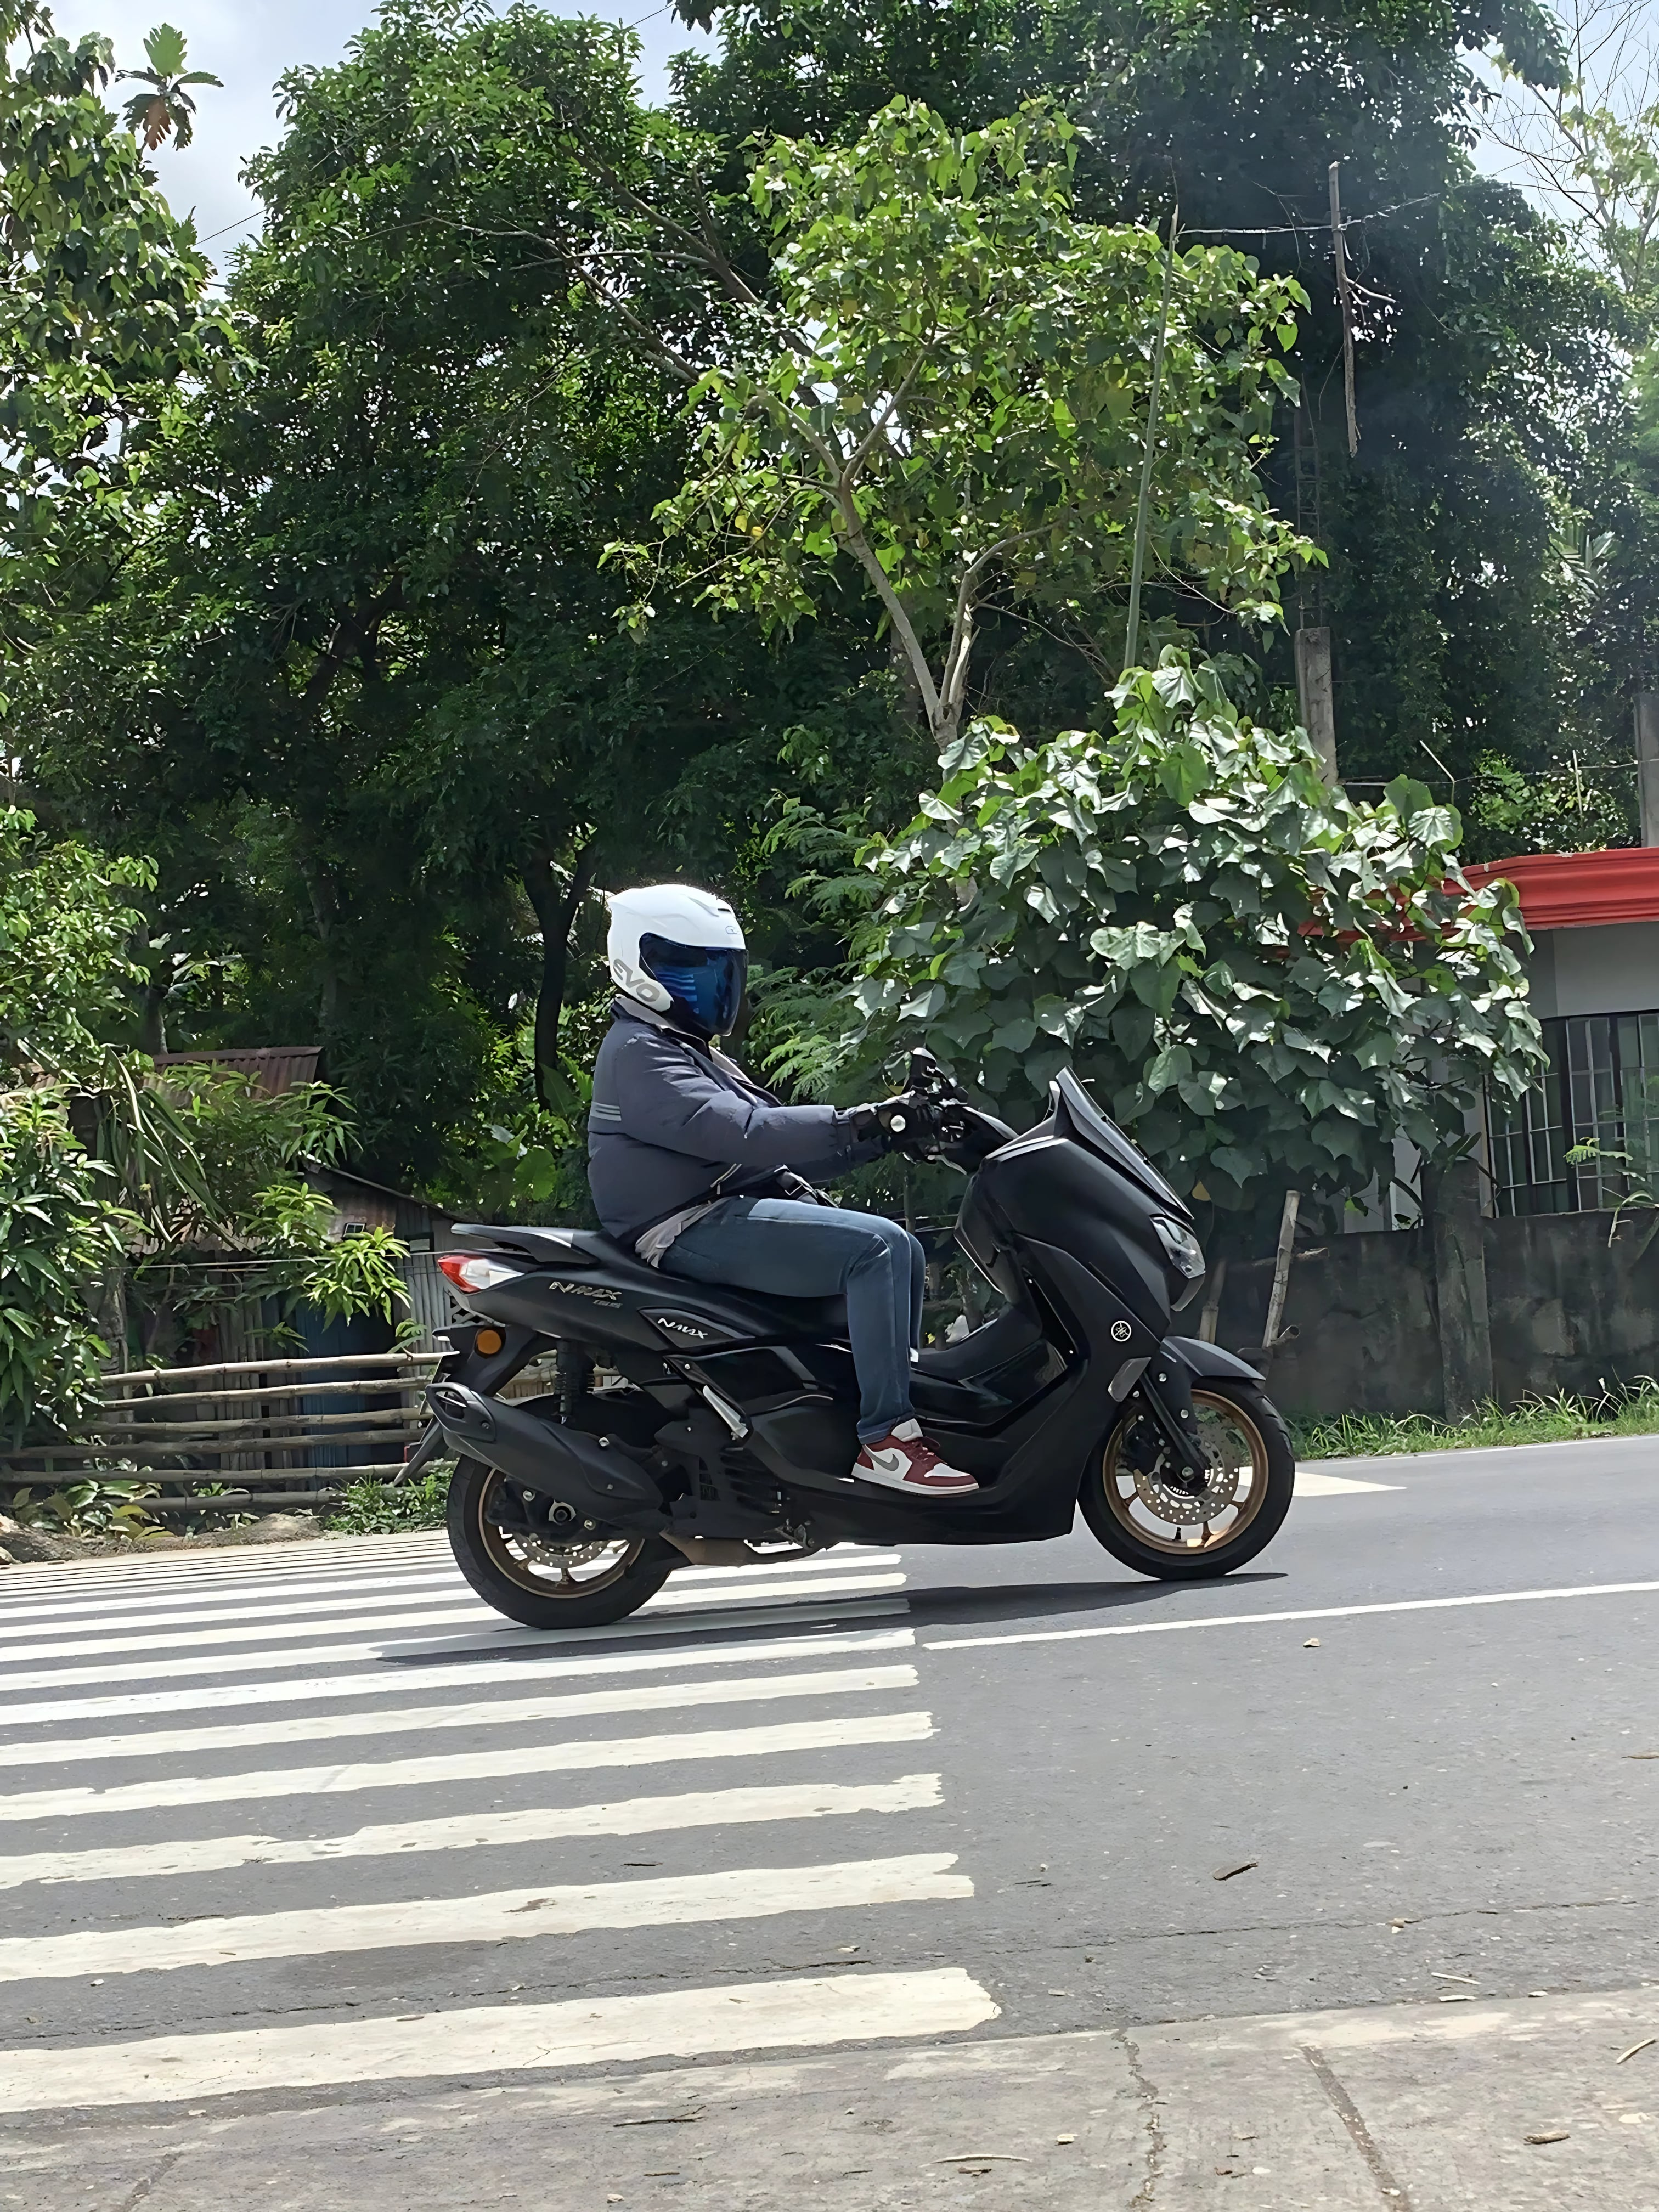
\includegraphics[width=0.35\textwidth]{figures/Fig 10.png} & 
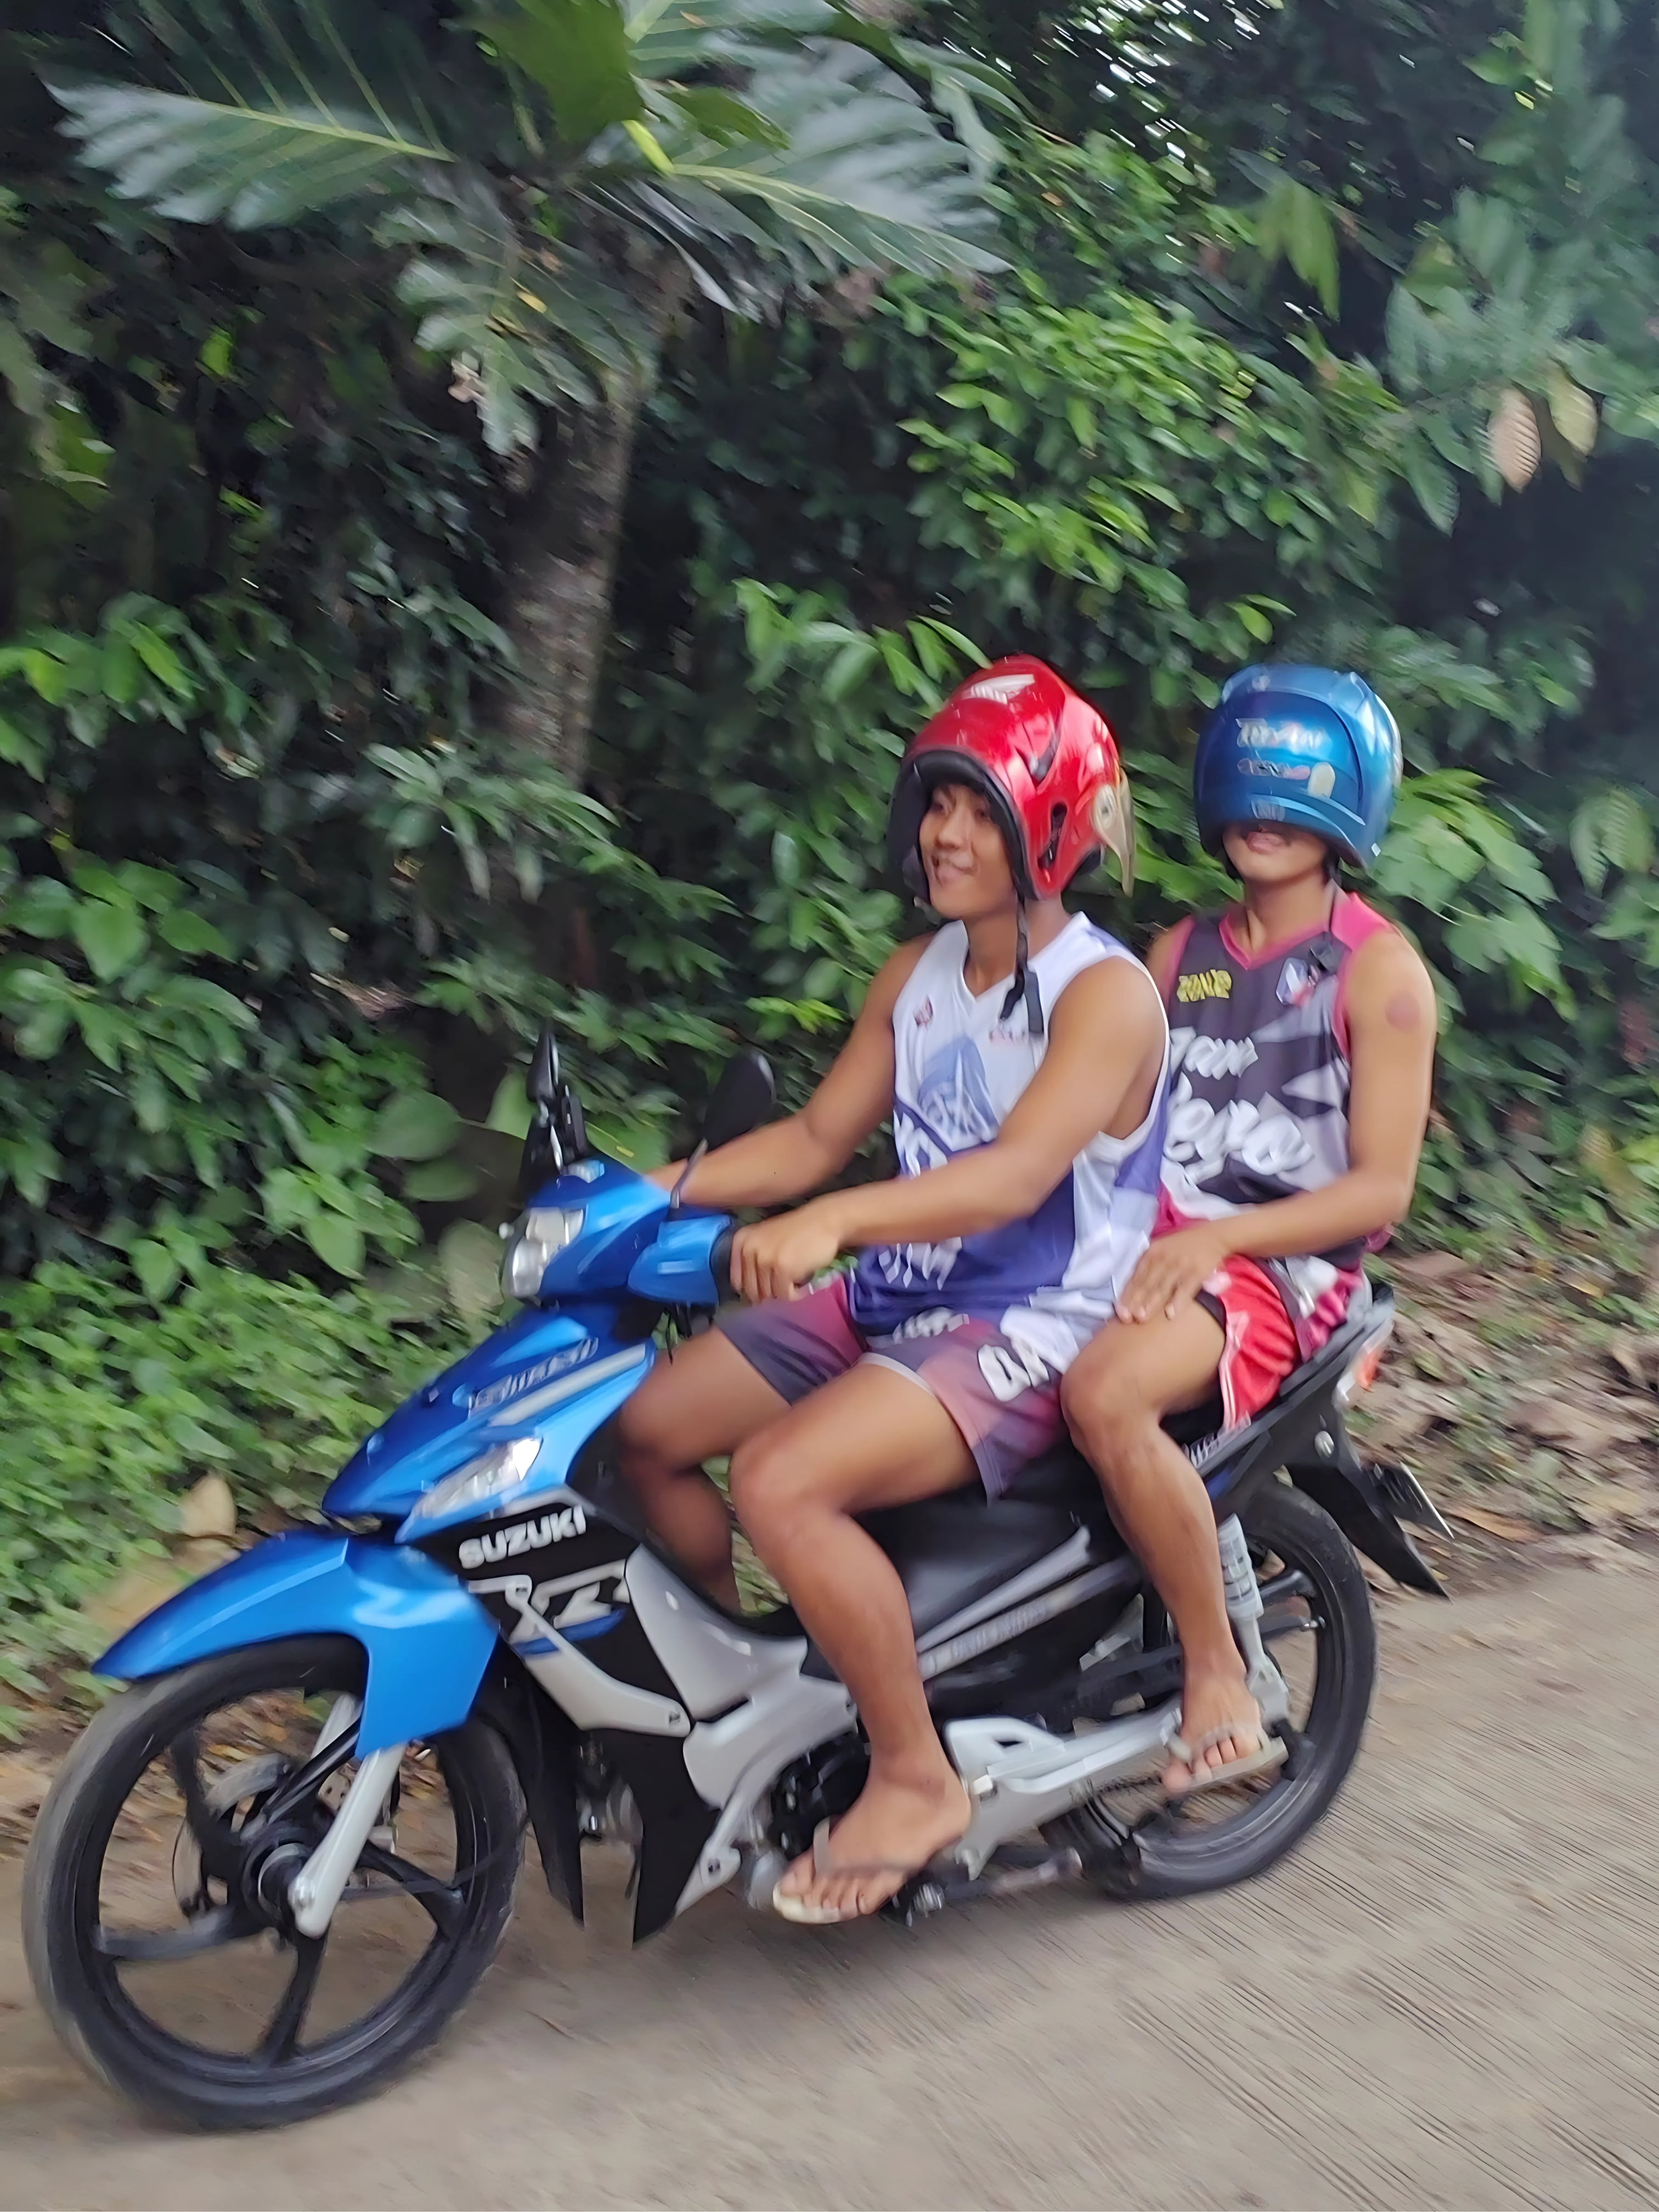
\includegraphics[width=0.35\textwidth]{figures/Fig 11.png} \\
\hline
\end{tabular}

\caption{Examples of Datasets.}
\label{fig:helmet_classification}
\end{figure}

\subsection{Data Pre-Processing}

\begin{figure}[ht]
    \centering
	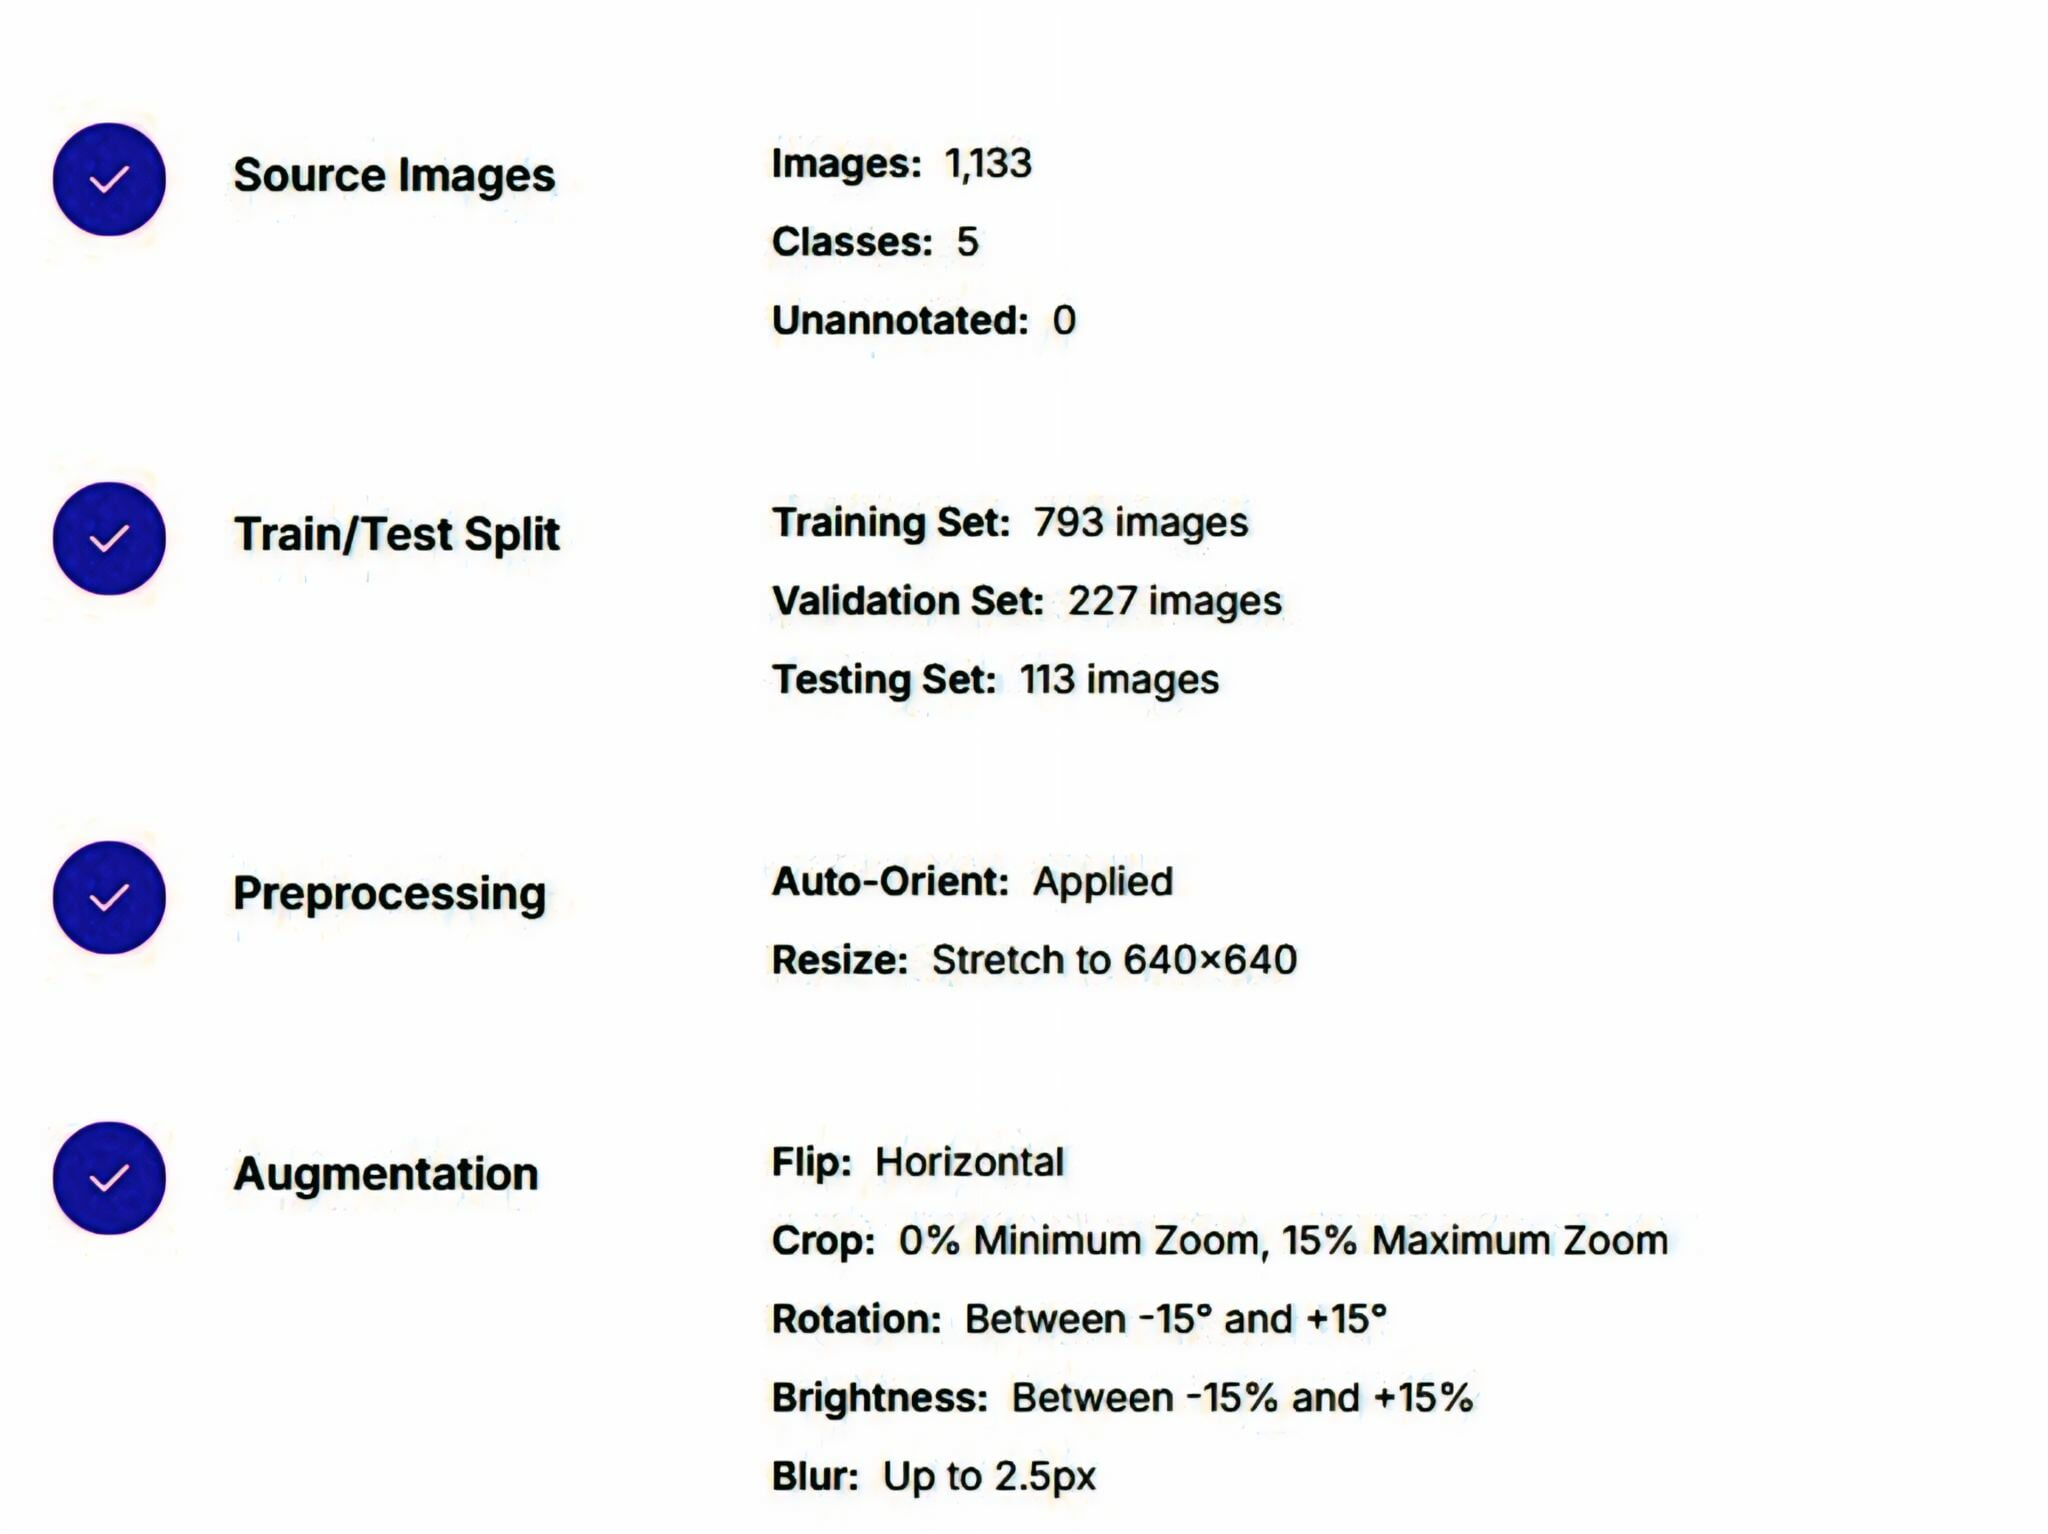
\includegraphics[width=0.85\textwidth]{figures/Fig 12.jpg}
	\caption[Data Pre-processing]{Data Pre-processing}
	\label{fig:data_preprocessing}
\end{figure}

A total of 1,133 images were collected and fully processed using Roboflow, where they were uploaded, annotated into five classes relevant to helmet compliance detection, and organized into a complete dataset. All images were properly labeled, ensuring no unannotated data remained. To support effective model training and evaluation, the dataset was divided into 793 images for training, 227 for validation, and 113 for testing. This split allowed the model to learn from the majority of the data while its accuracy was assessed on separate validation and testing sets.

In Roboflow, the images were preprocessed by applying auto-orientation to correct rotation errors and resizing them to 640×640 pixels, the standard input size required by the YOLOv8 model. To improve model performance and adaptability to real-world scenarios, several data augmentation techniques were applied. These included horizontal flipping to simulate different orientations, random cropping of up to 15\% to represent objects at varying distances, rotation adjustments between -15° and +15° to account for tilted camera angles, brightness variations of ±15\% to handle different lighting conditions, and blurring of up to 2.5 pixels to increase resilience to motion blur. These preprocessing and augmentation steps enriched the dataset, enabling the YOLOv8 model to generalize better and perform more reliably during testing and deployment.

\section{Model Training and Evaluation}
\noindent
The model was trained using a dataset with five classes: motorcycle, not motorcycle, person with no helmet, person with proper helmet, and person with wrong helmet use. The dataset was divided into training, validation, and test sets to evaluate the model. Before training, images were resized, normalized, and augmented using flipping, blurring, rotation, brightness changes, noise, and cropping to improve learning. The model was trained with the YOLOv8 algorithm for 150 epochs using batch processing, which allowed many images to be processed at once. It learned to detect and classify objects using the labeled bounding boxes. The model’s performance was measured using precision, recall, F1-score, and mean Average Precision (mAP) to show how accurately it detects helmet use and violations.

\begin{figure}[ht]
    \centering
	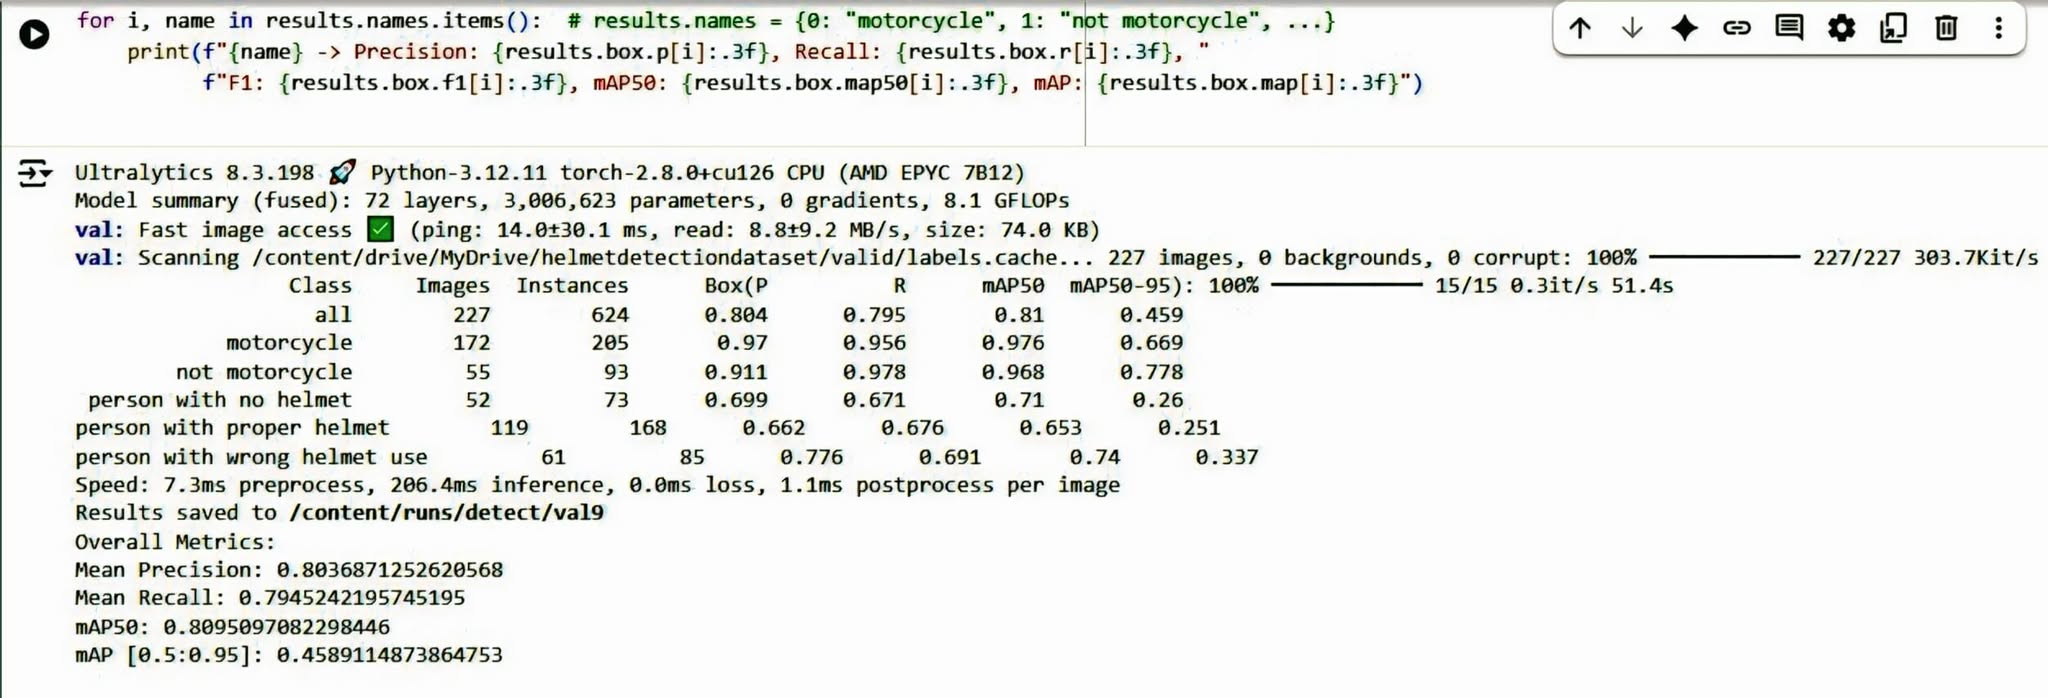
\includegraphics[width=0.85\textwidth]{figures/Fig 13.jpg}
	\caption[Model Training]{Model Training}
	\label{fig:model_training}
\end{figure}

\subsubsection{Model Evaluation}
\begin{figure}[ht]
    \centering
	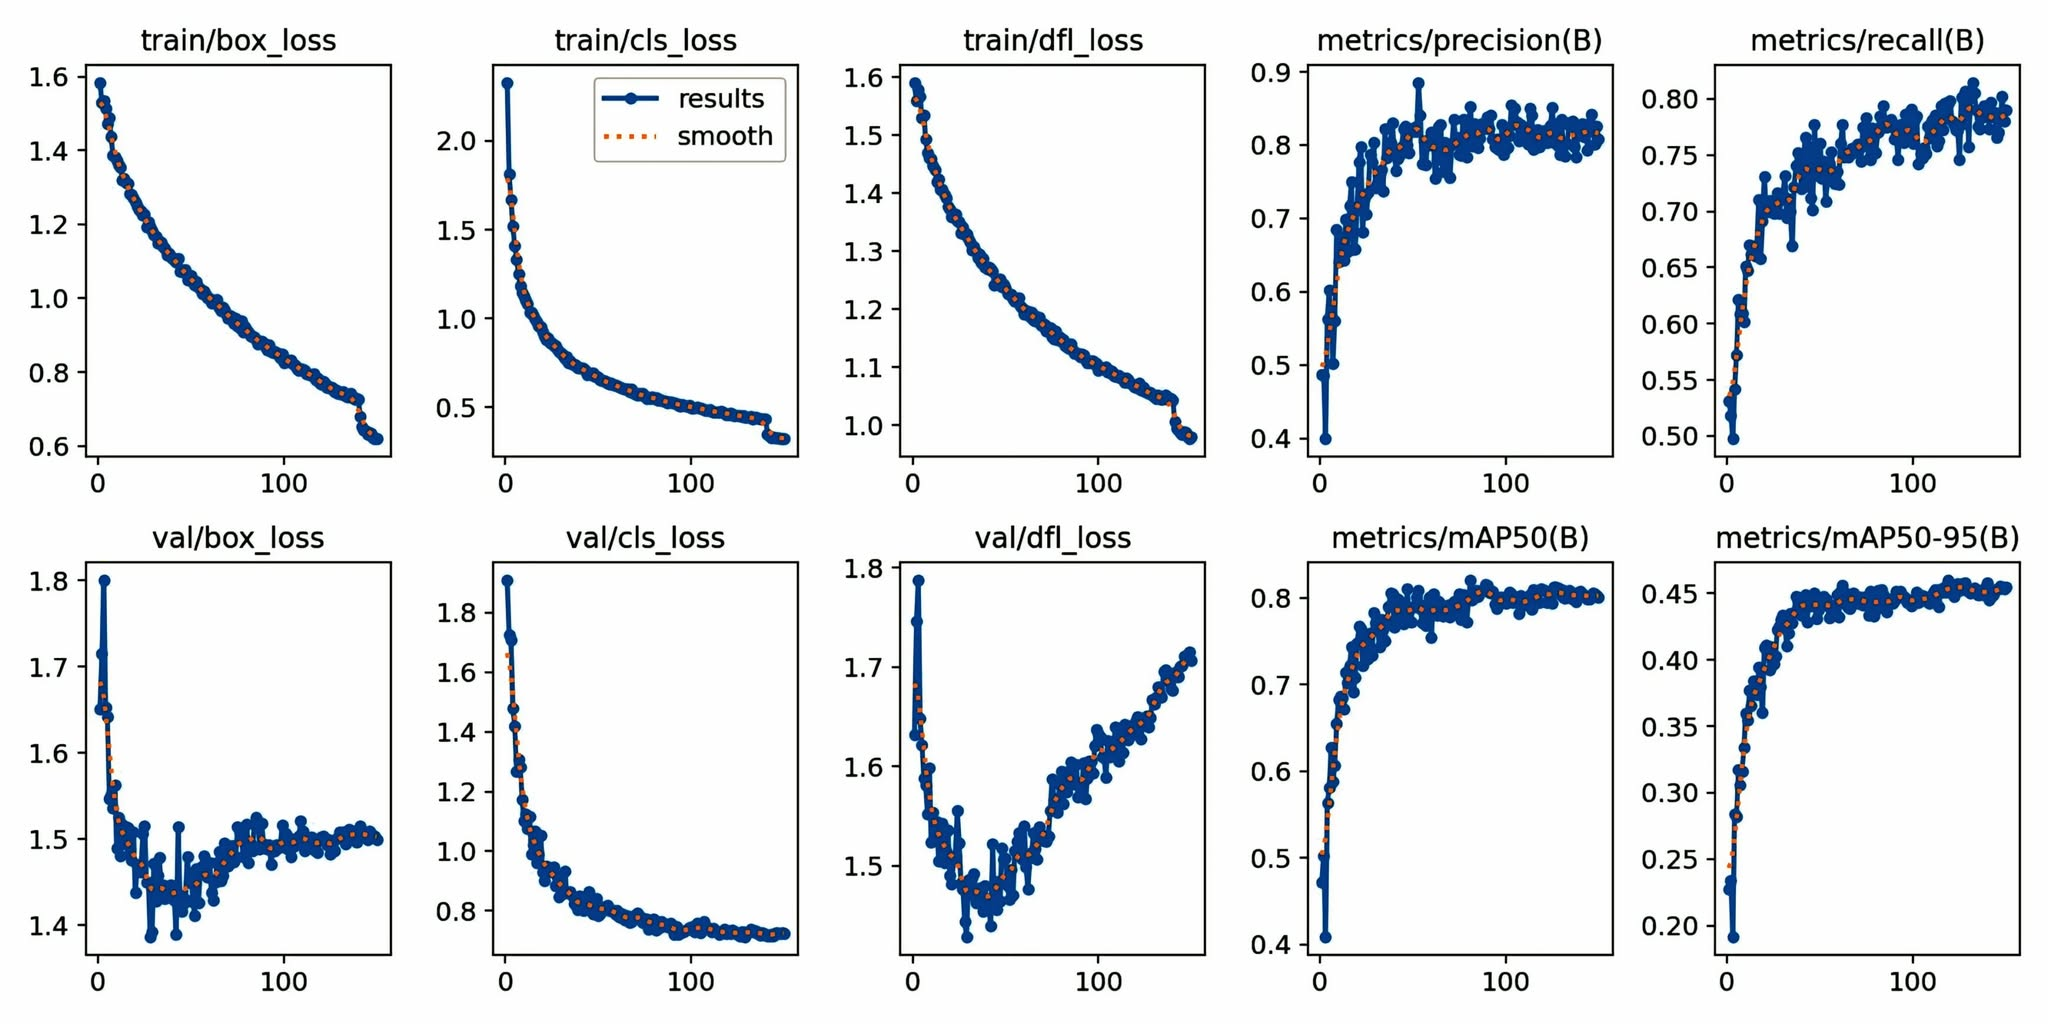
\includegraphics[width=0.85\textwidth]{figures/Fig 14.jpg}
	\caption[Model Evaluation]{Model Evaluation}
	\label{fig:model_evaluation}
\end{figure}

\noindent
Model evaluation results showing per-class performance on the validation dataset. The model achieved high precision and recall for detecting motorcycles, while helmet-related classes (“person with no helmet,” “person with proper helmet,” and “person with wrong helmet use”) had moderate performance. Overall mean precision and recall were approximately 80\%, with mAP50 at 0.81 and mAP@[0.5:0.95] at 0.46, indicating that the model is effective in identifying helmet compliance but has more difficulty with strict detection of helmet violations.

\subsubsection{Training Results}
\begin{figure}[ht]
    \centering
	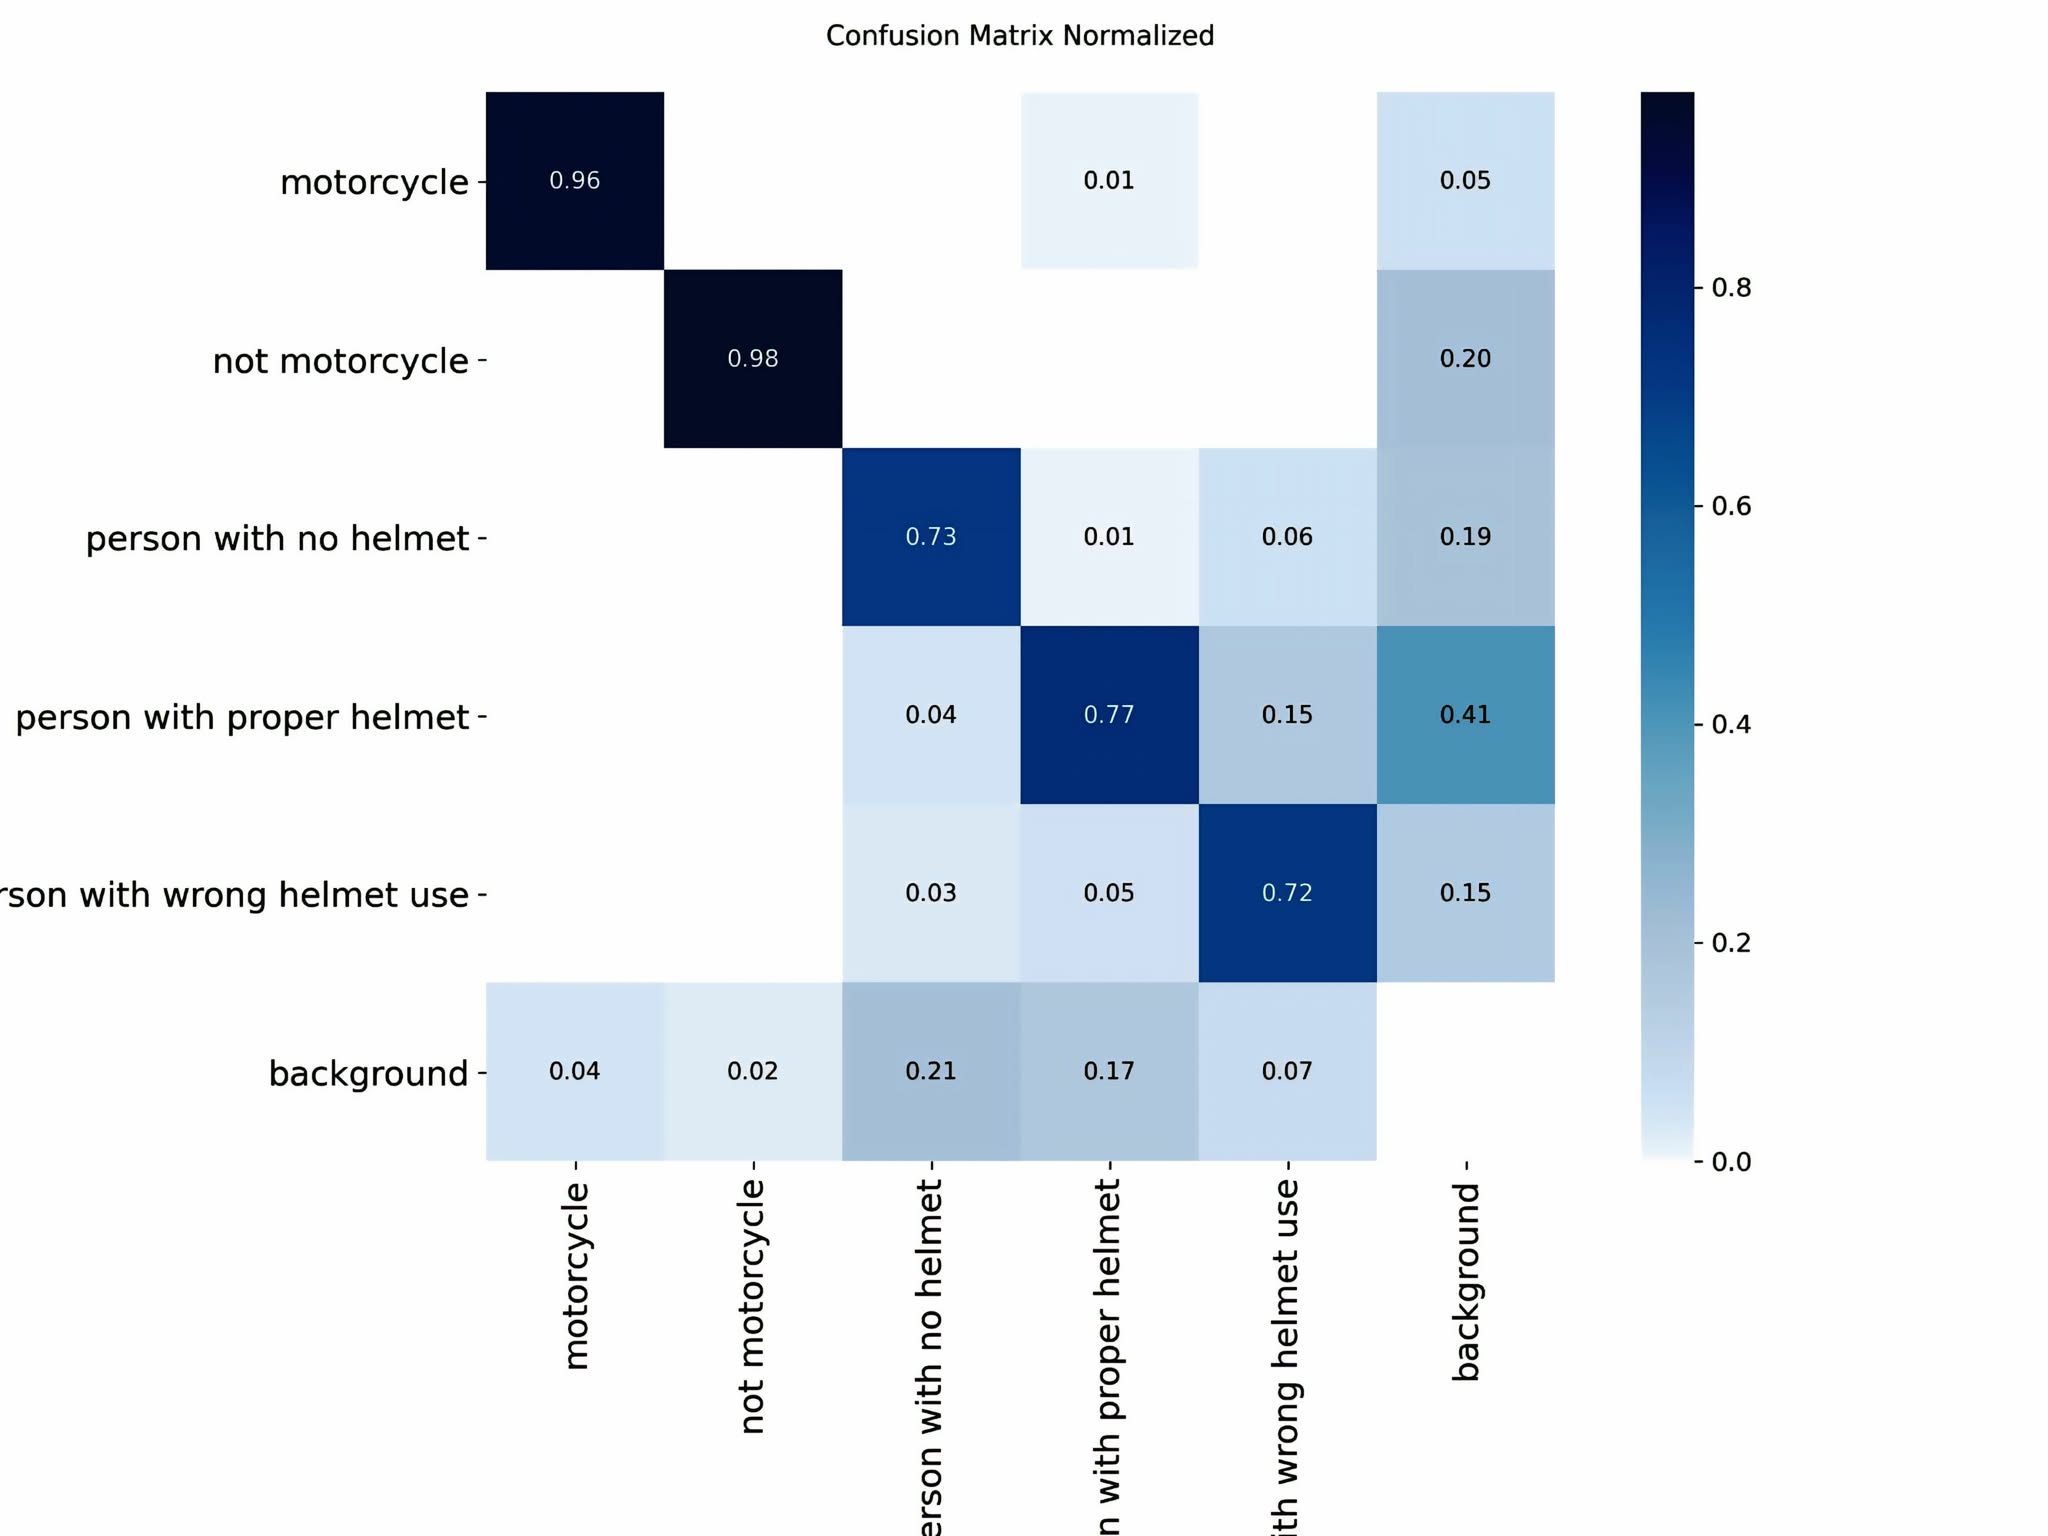
\includegraphics[width=0.85\textwidth]{figures/Fig 15.jpg}
	\caption[Training Results]{Training Results}
	\label{fig:training_results}
\end{figure}

\noindent
The training results show that the model learned effectively as the box, classification, and DFL losses decreased over time. Both precision and recall stabilized around 0.8, which means the model is good at correctly detecting objects and finding most of them. For overall detection performance, the model achieved about 0.8 mAP@50 and 0.45 mAP@50-95, showing strong accuracy though performance decreases under stricter evaluation. Validation results also suggest minor signs of overfitting, but the model still demonstrates reliable performance in identifying and classifying objects.

\subsubsection{Confusion Matrix}
\begin{figure}[ht]
    \centering
	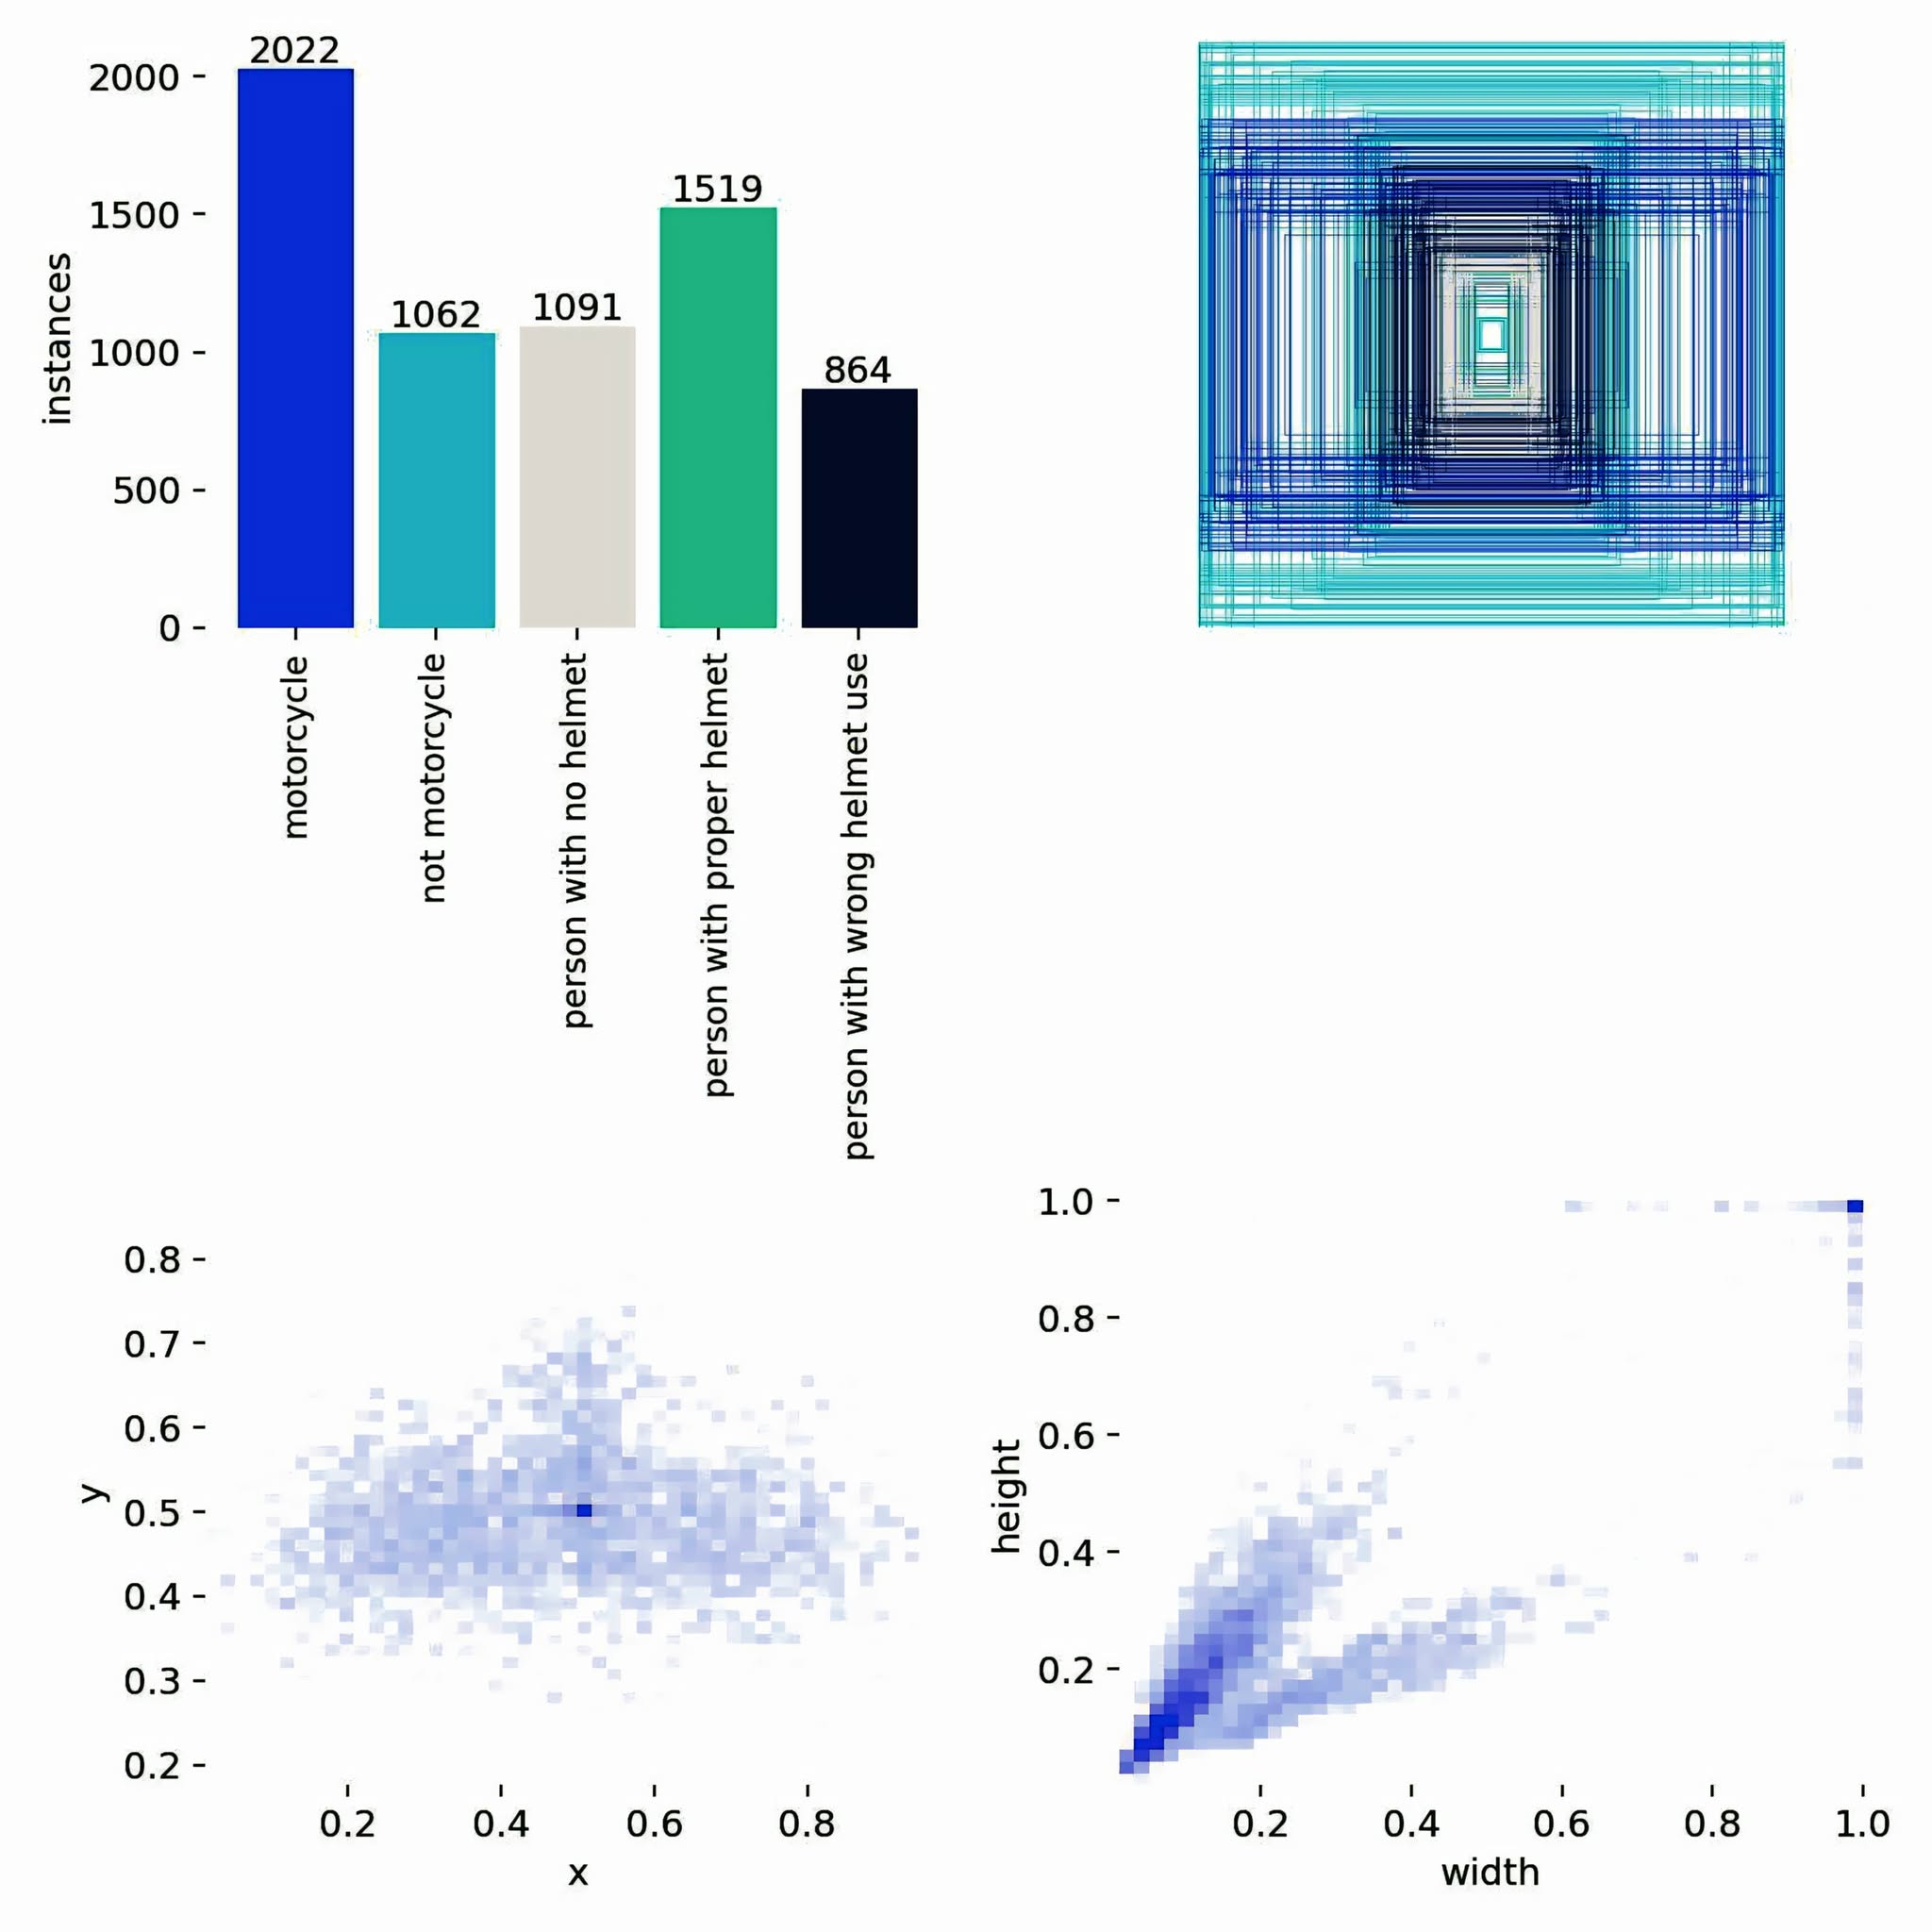
\includegraphics[width=0.85\textwidth]{figures/Fig 16.jpg}
	\caption[Confusion Matrix]{Confusion Matrix}
	\label{fig:confusion_matrix}
\end{figure}

\noindent
The confusion matrix shows that the model performs very well in identifying motorcycles (96\%) and non-motorcycles (98\%). However, it has moderate accuracy in detecting helmet-related classes, with 73\% for no helmet, 77\% for proper helmet, and 72\% for wrong helmet use. Misclassifications often occur between proper and wrong helmet use, or between no helmet and background. This means the model is strong in detecting motorcycles but still struggles with fine distinctions in helmet usage and separating persons from the background.

\subsubsection{Dataset Visualization}
\begin{figure}[ht]
    \centering
	\includegraphics[width=0.85\textwidth]{figures/Fig 17.jpg}
	\caption[Dataset Visualization]{Dataset Visualization}
	\label{fig:dataset_visualization}
\end{figure}

\noindent
The dataset visualization highlights the distribution and positioning of the annotated classes. The bar chart shows that motorcycles (2022 instances) and persons with proper helmet use (1519 instances) dominate the dataset, while wrong helmet use (864 instances) is the least represented, indicating some class imbalance. Persons without helmets (1062) and non-motorcycle objects (1091) also contribute significantly to the dataset. The bounding box heatmap suggests that most objects are centered in the images, which may help the model focus on relevant regions. Additionally, the width and height distribution indicates that many objects are relatively small, with fewer larger ones, which may influence detection accuracy. Overall, the dataset provides a strong foundation for training but requires attention to class imbalance to ensure balanced performance across all categories.

\subsubsection{Box Curve}
\begin{figure}[H]
\centering
\begin{tabular}{cc}
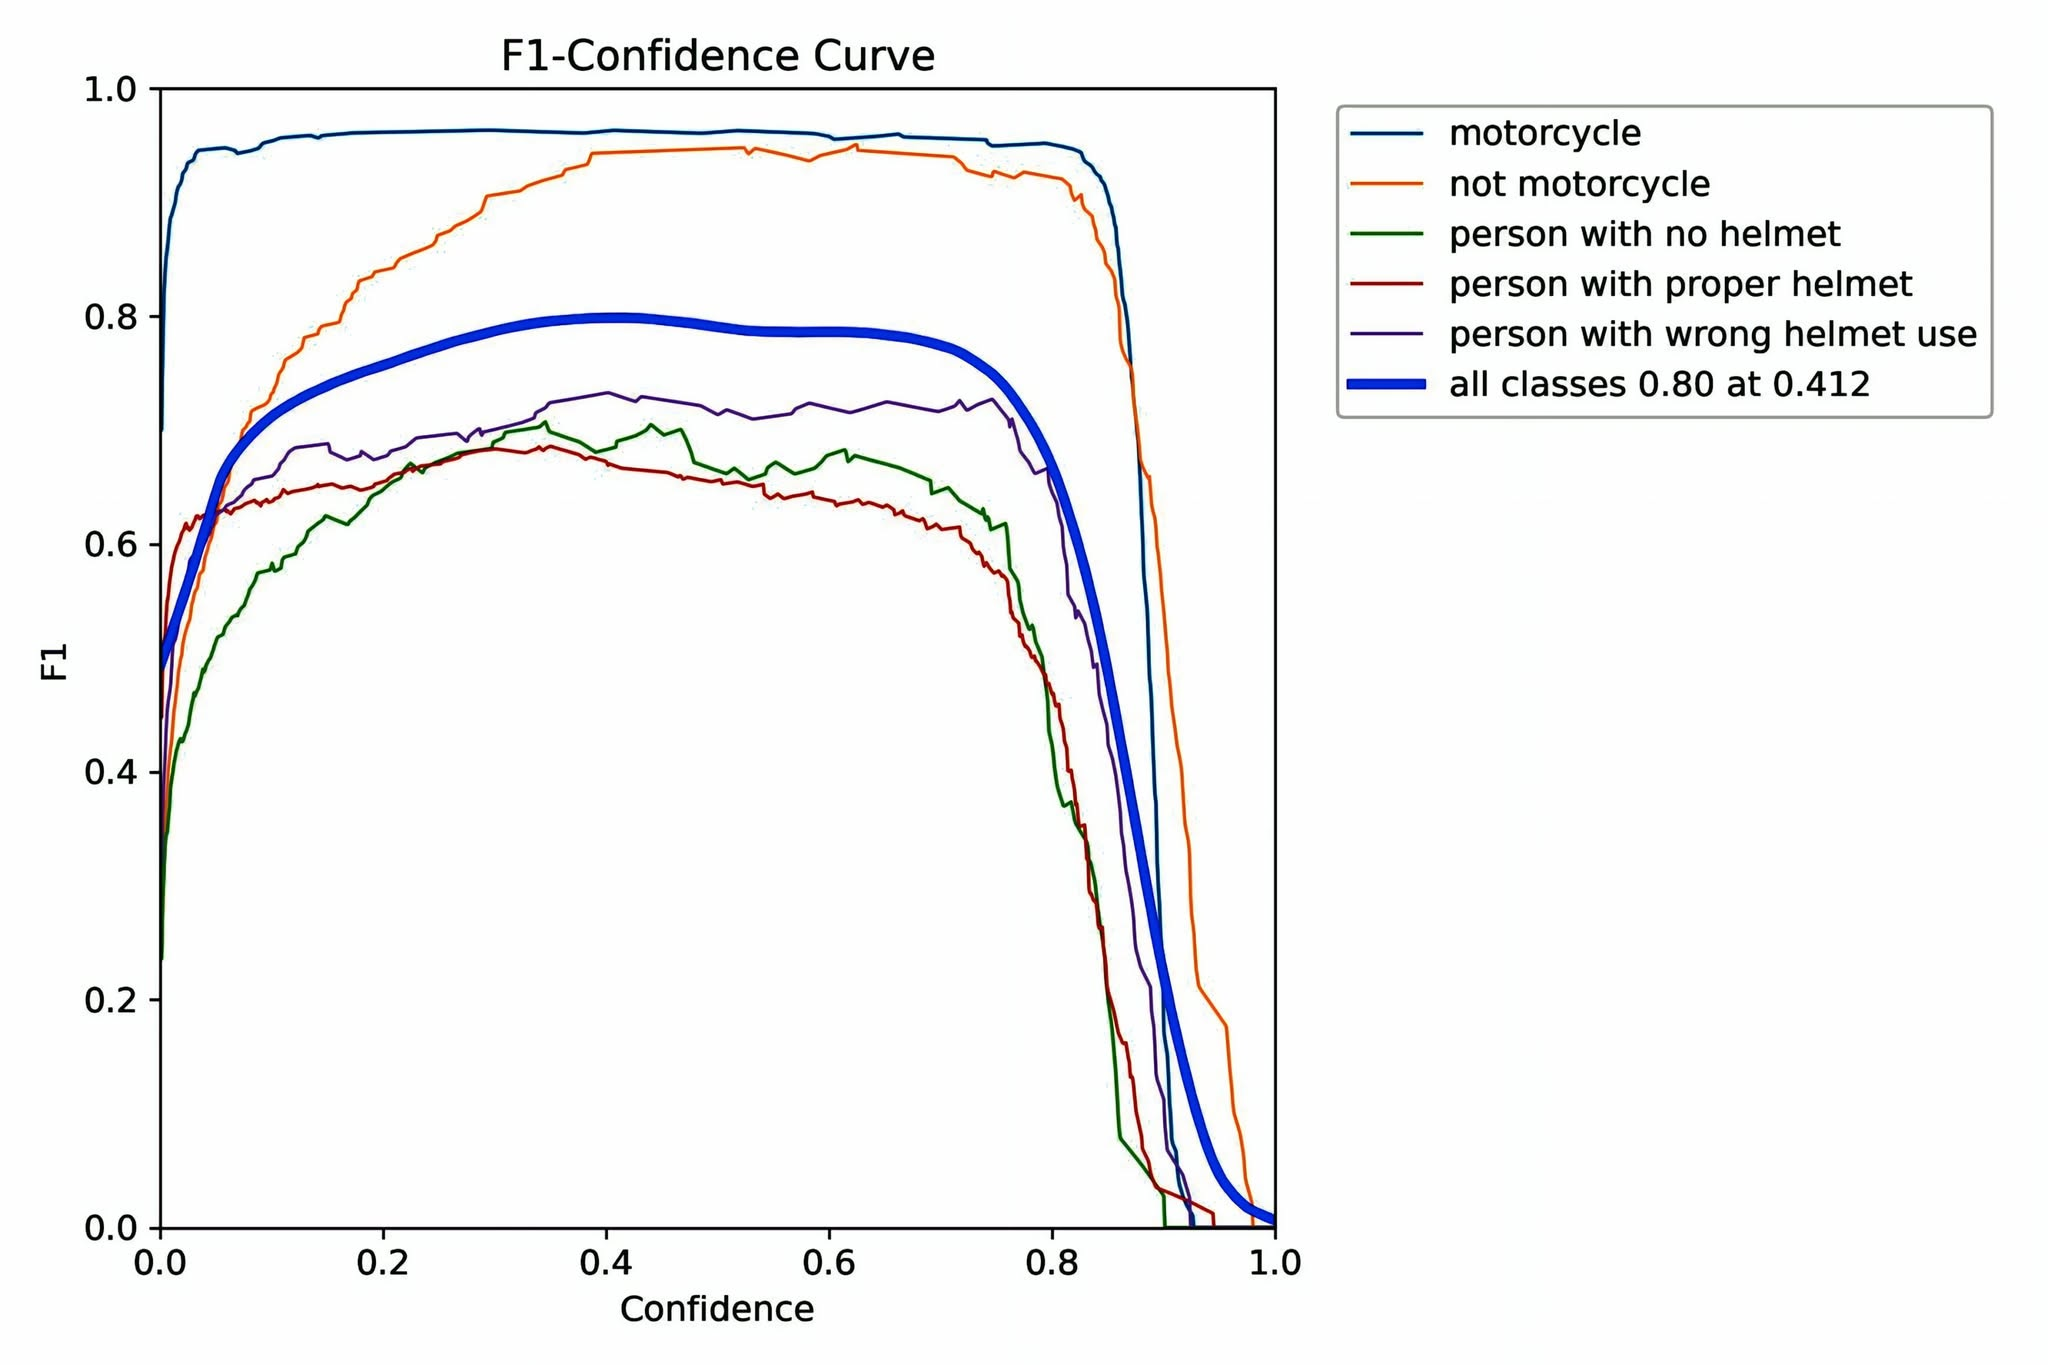
\includegraphics[width=0.45\textwidth]{figures/Fig18a.jpg} &
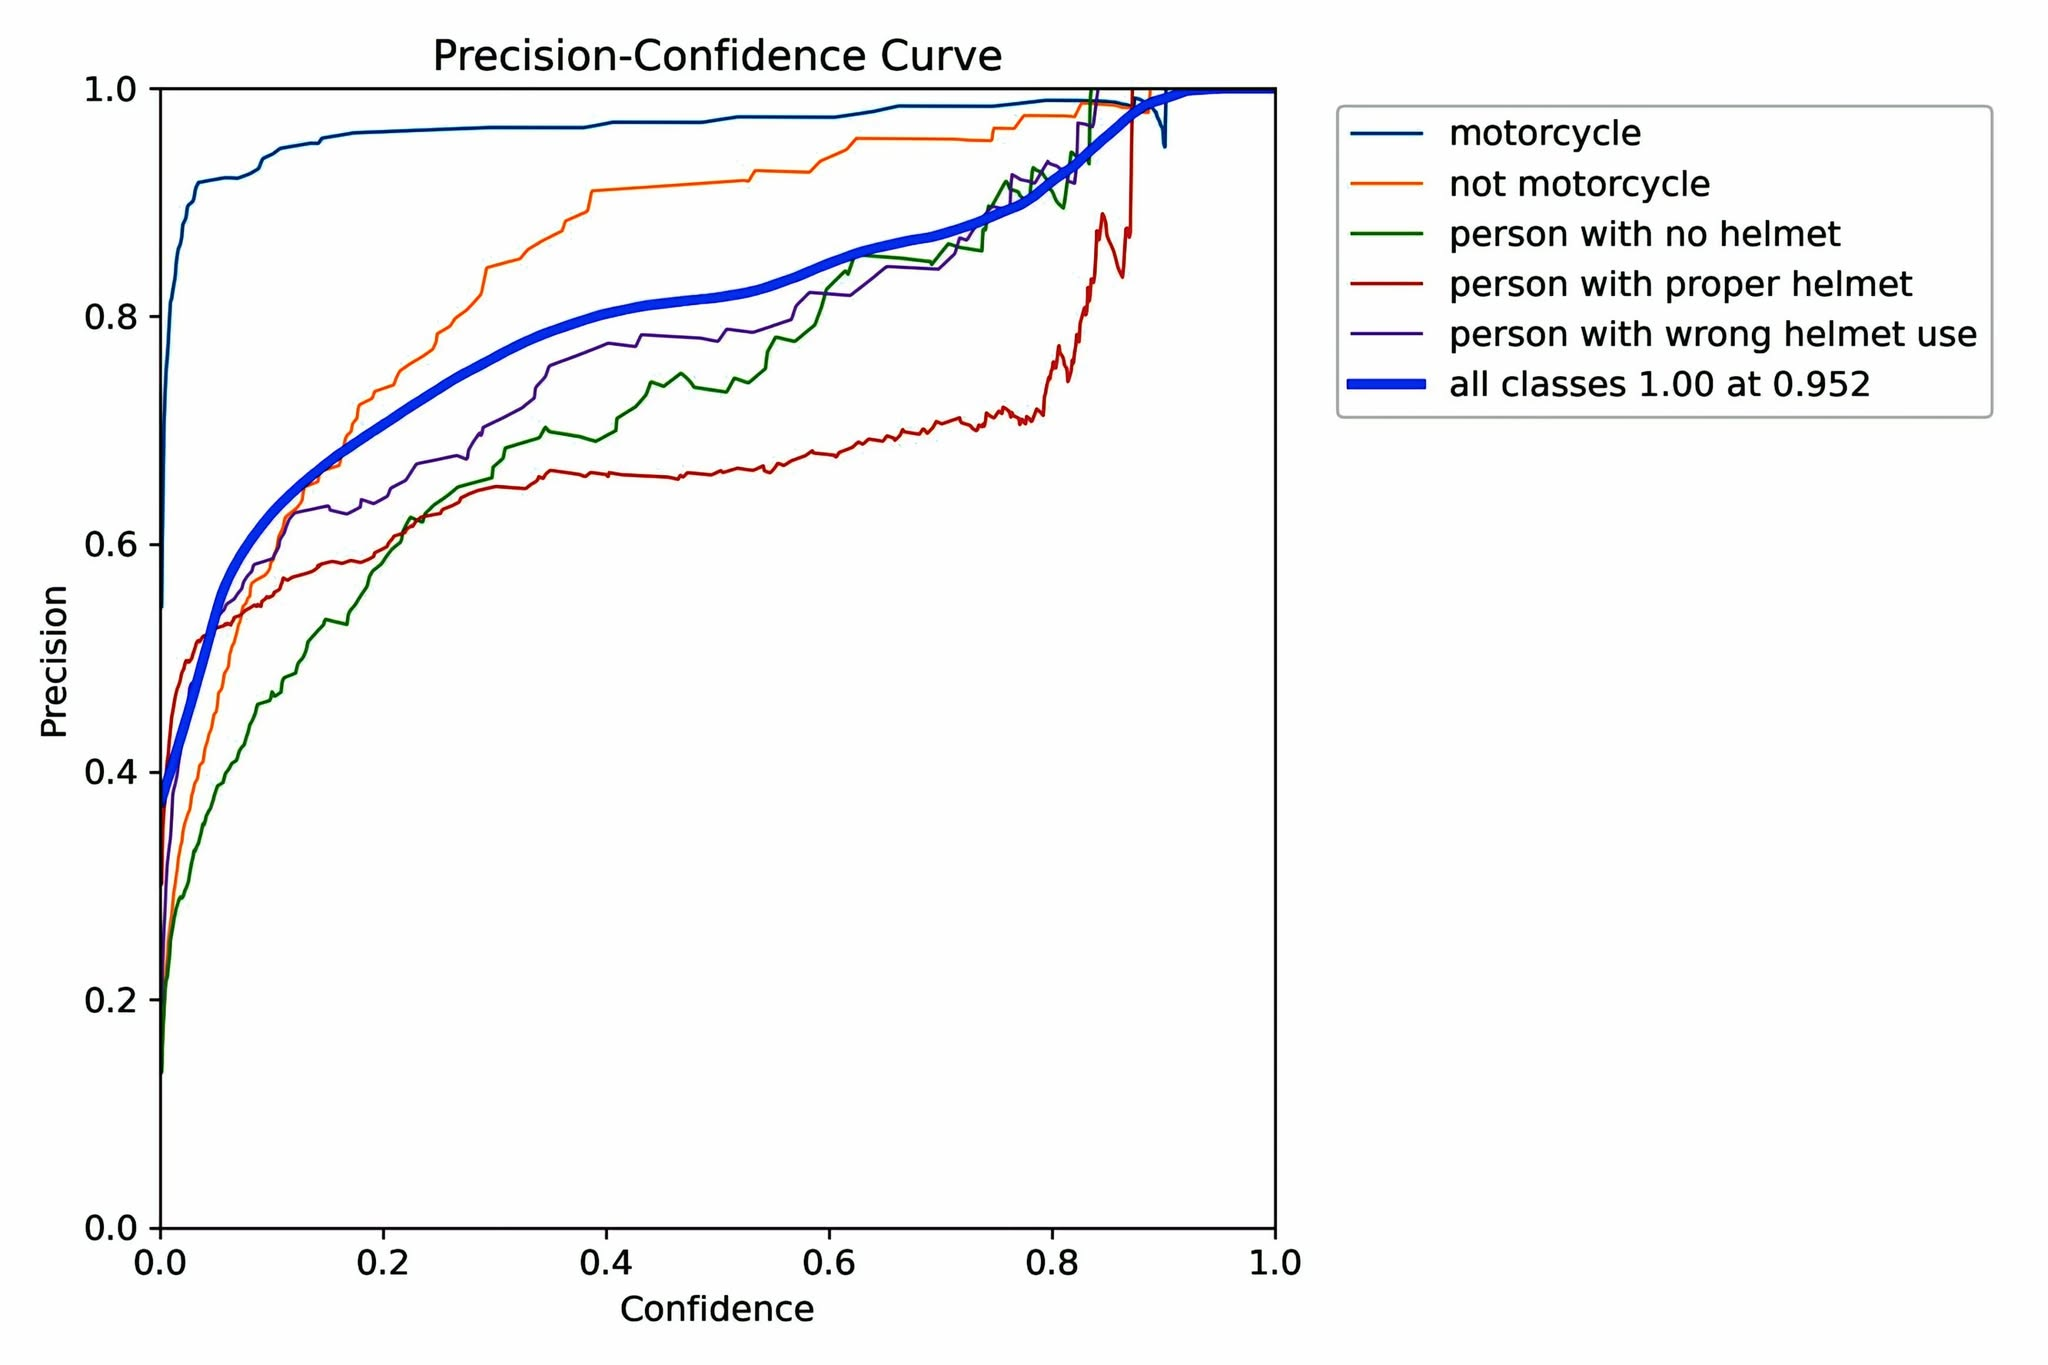
\includegraphics[width=0.45\textwidth]{figures/Fig18b.jpg} \\
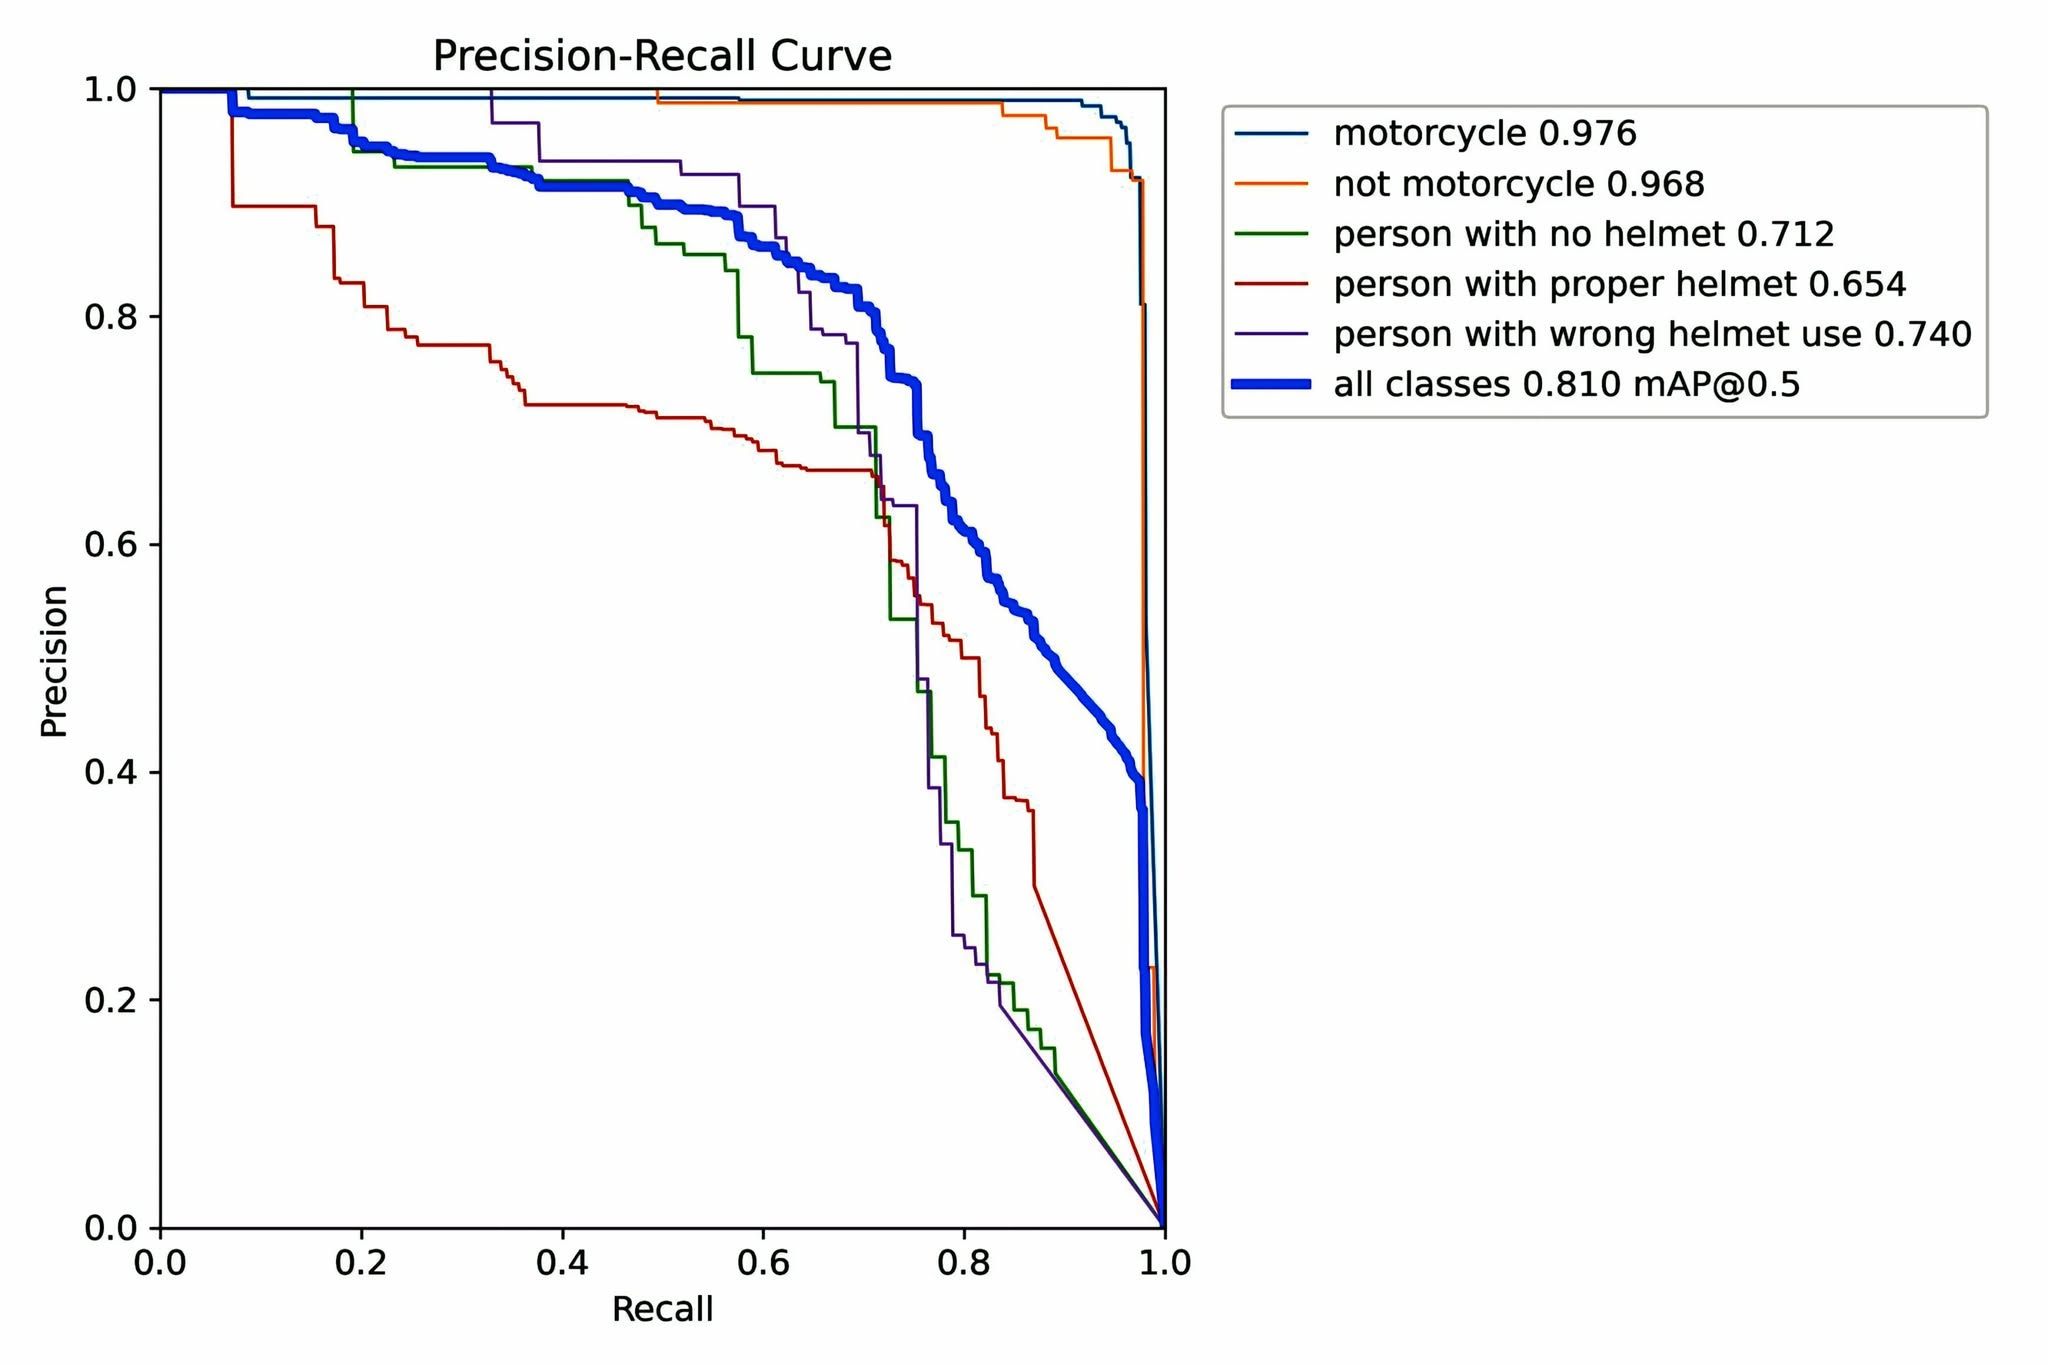
\includegraphics[width=0.45\textwidth]{figures/Fig18c.jpg} &
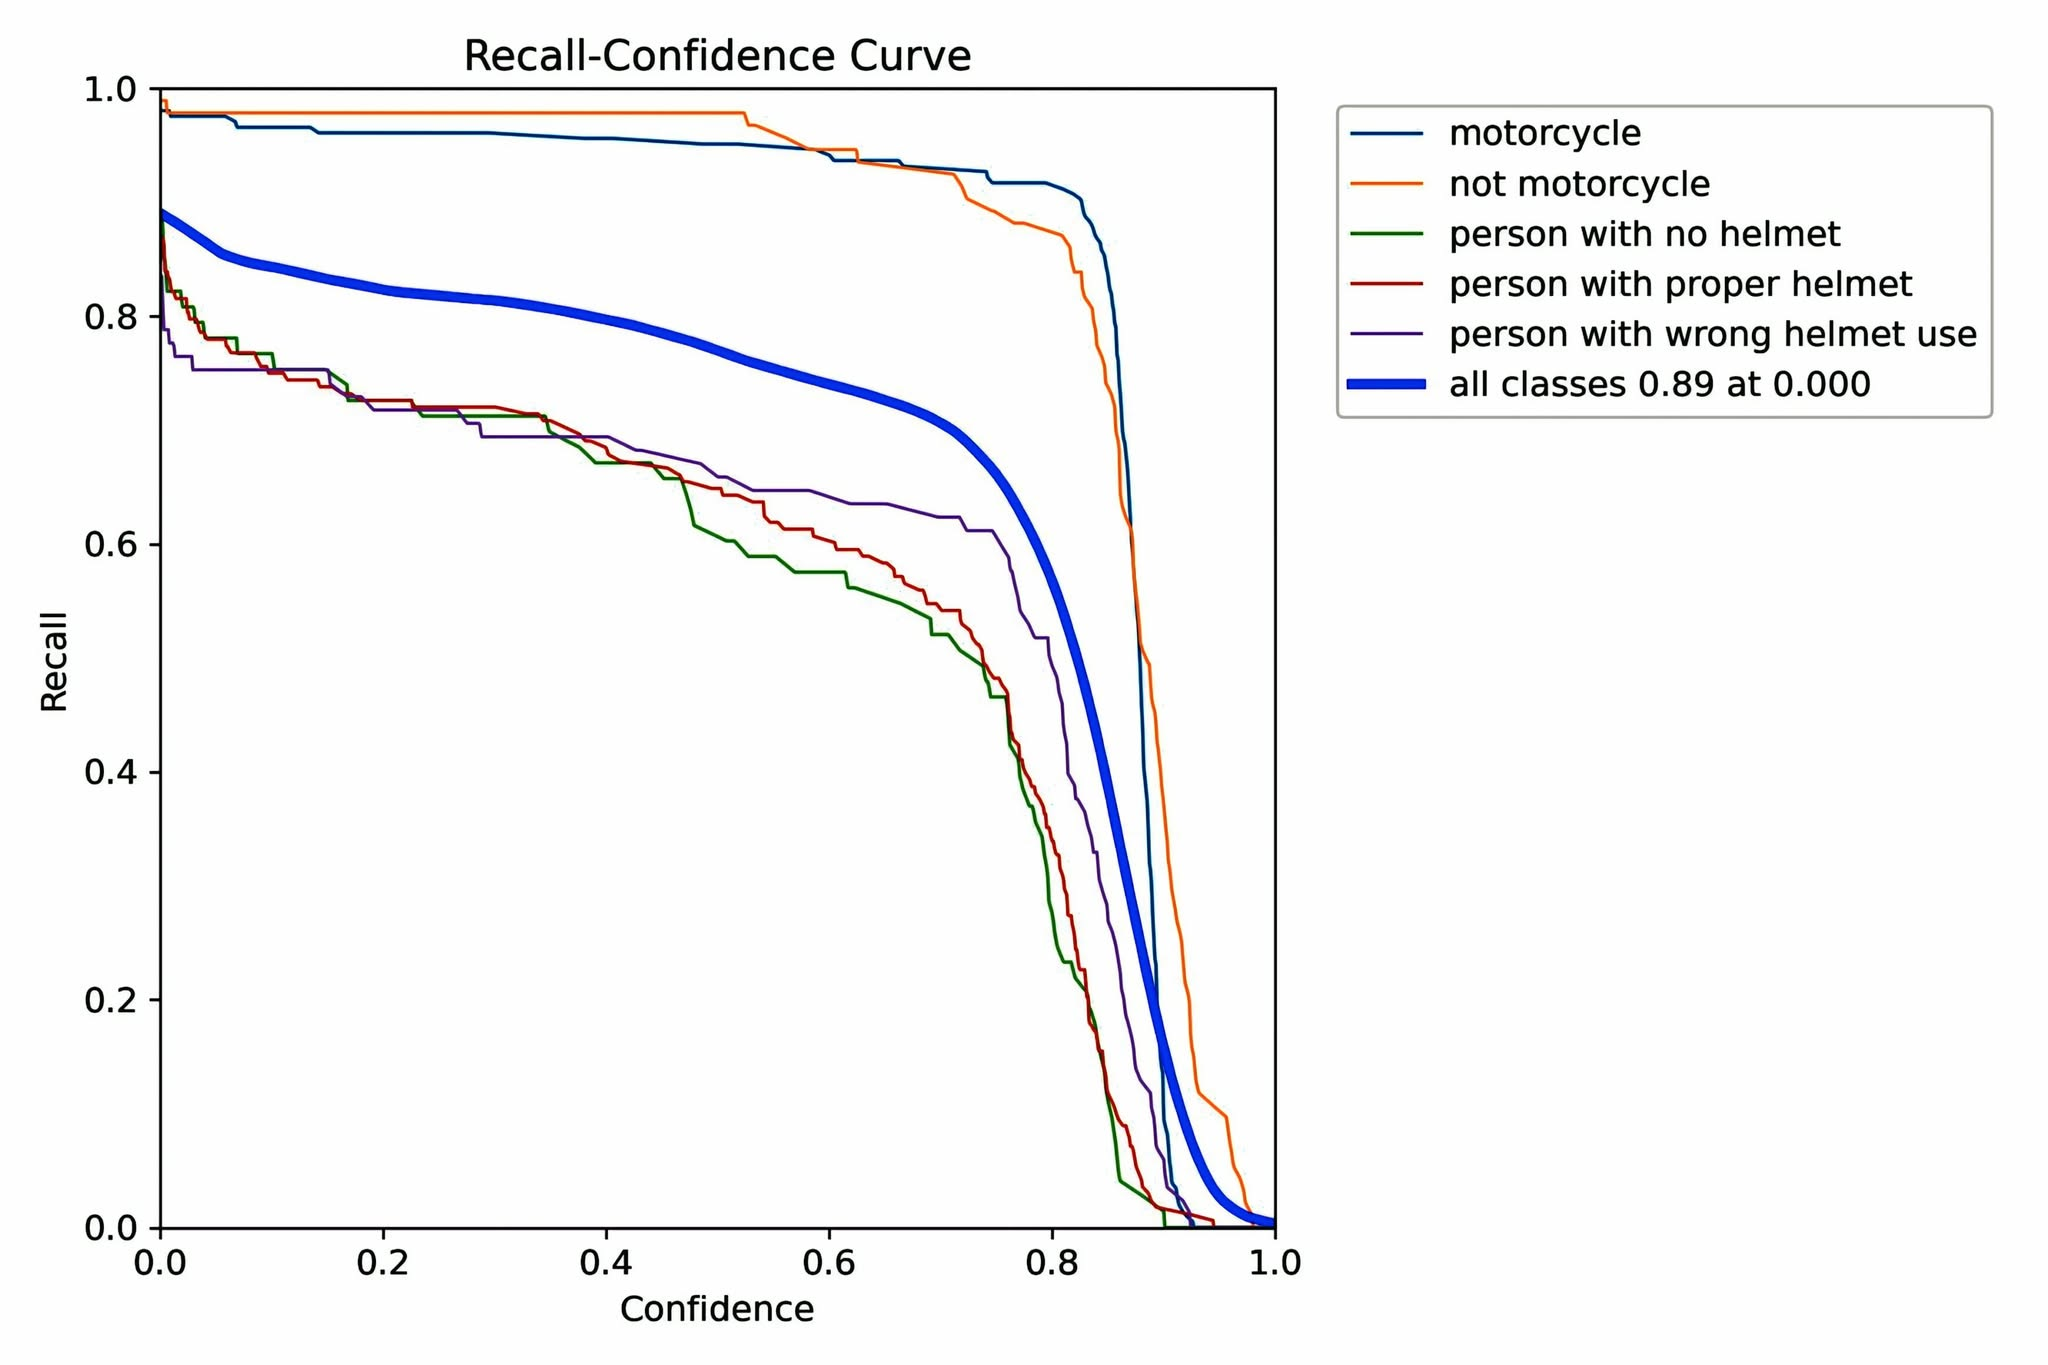
\includegraphics[width=0.45\textwidth]{figures/Fig18d.jpg} \\
\end{tabular}
\caption{Box Curve Results}
\label{fig:box_curve}
\end{figure}

\noindent
The performance evaluation graphs provide insights into how well the model detects motorcycles and helmet usage. In the F1-Confidence Curve (Graph A), the model achieves its best balance between precision and recall at a confidence threshold of around 0.41, with an overall F1 score of 0.80. The classes motorcycle and not motorcycle consistently achieve higher F1 scores compared to the helmet-related classes. The Precision-Confidence Curve (Graph B) shows that precision improves as the confidence threshold increases, with motorcycle and not motorcycle approaching near-perfect precision at high thresholds, while helmet-related classes such as proper helmet use and no helmet show lower precision values. The Precision-Recall Curve (Graph C) highlights that the model performs very well in detecting motorcycles (0.976) and non-motorcycles (0.968), but has lower average precision scores for helmet-related categories, with no helmet at 0.712, proper helmet use at 0.654, and wrong helmet use at 0.740, resulting in an overall mean Average Precision (mAP@0.5) of 0.810. Lastly, the Recall-Confidence Curve (Graph D) indicates that recall is highest at lower confidence thresholds, with an overall recall of 0.89, but gradually decreases as confidence increases, showing that while the model can detect most objects at low thresholds, higher thresholds ensure more reliable but fewer detections.

%=======================================================%
%%%%% Do not delete this part %%%%%%
\clearpage

\printbibliography[heading=subbibintoc, title={\texorpdfstring{\centering}{} Notes}]
\end{refsection}
